% Capitolul 10: VaR, ES și backtesting
% Statistica piețelor financiare -- Program de licență, Academia de Studii Economice din București
% GENERAT de latex/build_chapter10.py -- modificați generatorul, nu acest fișier.

\newcommand{\coursename}{Statistica piețelor financiare}
\def\sfmlang{ro}
% Preambul comun SFM -- Statistica piețelor financiare / Statistics of Financial Markets (Beamer, 16:9)
% Același design ca MFM. Înainte de % Preambul comun SFM -- Statistica piețelor financiare / Statistics of Financial Markets (Beamer, 16:9)
% Același design ca MFM. Înainte de % Preambul comun SFM -- Statistica piețelor financiare / Statistics of Financial Markets (Beamer, 16:9)
% Același design ca MFM. Înainte de \input{../../latex/preamble} se definește
%   \newcommand{\coursename}{Statistics of Financial Markets}      (EN)
%   \newcommand{\coursename}{Statistica piețelor financiare}       (RO)  și  \def\sfmlang{ro}
% Fișierele .tex se află în EN/Courses, EN/Seminars, RO/Cursuri, RO/Seminarii (două niveluri sub rădăcină).
% Deck-urile sînt generate de latex/build_chapterN.py / build_seminarN.py (vezi latex/sfm_build.py).

\documentclass[9pt, aspectratio=169, t]{beamer}
\providecommand{\coursename}{Statistics of Financial Markets}

% Ensure content fits on slides
\setbeamersize{text margin left=8mm, text margin right=8mm}

%=============================================================================
% THEME AND STYLE CONFIGURATION
%=============================================================================
\usetheme{default}
% Using default theme for clean header/footer control

% Color Palette (matching Redispatch PDF)
\definecolor{MainBlue}{RGB}{26, 58, 110}
\definecolor{AccentBlue}{RGB}{26, 58, 110}
\definecolor{IDAred}{RGB}{205, 0, 0}
\definecolor{DarkGray}{RGB}{51, 51, 51}
\definecolor{MediumGray}{RGB}{128, 128, 128}
\definecolor{LightGray}{RGB}{248, 248, 248}
\definecolor{VeryLightGray}{RGB}{235, 235, 235}
\definecolor{KeynoteGray}{RGB}{218, 218, 218}
\definecolor{SectionGray}{RGB}{120, 120, 120}
\definecolor{FooterGray}{RGB}{100, 100, 100}
\definecolor{Crimson}{RGB}{220, 53, 69}
\definecolor{Forest}{RGB}{46, 125, 50}
\definecolor{Amber}{RGB}{181, 133, 63}
\definecolor{Orange}{RGB}{230, 126, 34}
\definecolor{Purple}{RGB}{142, 68, 173}

% Gradient background (exact Keynote 315° gradient: white to RGB 218,218,218)
\setbeamertemplate{background}{%
    \begin{tikzpicture}[remember picture, overlay]
        \shade[shading=axis, shading angle=315,
        top color=white, bottom color=KeynoteGray]
        (current page.south west) rectangle (current page.north east);
    \end{tikzpicture}%
}
% Fallback solid color for compatibility
\setbeamercolor{background canvas}{bg=}

\setbeamercolor{palette primary}{bg=MainBlue, fg=white}
\setbeamercolor{palette secondary}{bg=MainBlue!85, fg=white}
\setbeamercolor{palette tertiary}{bg=MainBlue!70, fg=white}
\setbeamercolor{structure}{fg=MainBlue}
\setbeamercolor{title}{fg=IDAred}
\setbeamercolor{frametitle}{fg=IDAred, bg=}
\setbeamercolor{block title}{bg=MainBlue, fg=white}
\setbeamercolor{block body}{bg=VeryLightGray, fg=DarkGray}
\setbeamercolor{block title alerted}{bg=Crimson, fg=white}
\setbeamercolor{block body alerted}{bg=Crimson!8, fg=DarkGray}
\setbeamercolor{block title example}{bg=Forest, fg=white}
\setbeamercolor{block body example}{bg=Forest!8, fg=DarkGray}
\setbeamercolor{item}{fg=MainBlue}

% Footer colors (override Madrid theme blue)
\setbeamercolor{author in head/foot}{fg=FooterGray, bg=}
\setbeamercolor{title in head/foot}{fg=FooterGray, bg=}
\setbeamercolor{date in head/foot}{fg=FooterGray, bg=}
\setbeamercolor{section in head/foot}{fg=FooterGray, bg=}
\setbeamercolor{subsection in head/foot}{fg=FooterGray, bg=}

% Bullet styles (apply everywhere including blocks)
\setbeamertemplate{itemize item}{\color{MainBlue}$\boxdot$}
\setbeamertemplate{itemize subitem}{\color{MainBlue}$\blacktriangleright$}
\setbeamertemplate{itemize subsubitem}{\color{MainBlue}\tiny$\bullet$}
\setbeamertemplate{itemize/enumerate body begin}{\normalsize}
\setbeamertemplate{itemize/enumerate subbody begin}{\normalsize}

% Item spacing - compact style
\setlength{\leftmargini}{10pt}       % Level 1: minimal indent
\setlength{\leftmarginii}{10pt}      % Level 2: minimal additional indent
% Compact list spacing (zero extra space before/after lists in blocks)
\makeatletter
\def\@listi{\leftmargin\leftmargini \topsep 0pt \parsep 0pt \itemsep 0pt}
\def\@listii{\leftmargin\leftmarginii \topsep 0pt \parsep 0pt \itemsep 0pt}
\makeatother

\setbeamertemplate{navigation symbols}{}

%=============================================================================
% CUSTOM HEADLINE
%=============================================================================
\setbeamertemplate{headline}{%
    \vskip10pt%
    \hbox to \paperwidth{%
        \hskip0.5cm%
        {\small\color{FooterGray}\renewcommand{\hyperlink}[2]{##2}\insertsectionhead}%
        \hfill%
        \textcolor{FooterGray}{\small\insertframenumber}%
        \hskip0.5cm%
    }%
    \vskip4pt%
    {\color{FooterGray}\hrule height 0.4pt}%
}

%=============================================================================
% CUSTOM FOOTER
%=============================================================================
\usepackage{fontawesome5}

\setbeamertemplate{footline}{%
    {\color{FooterGray}\hrule height 0.4pt}%
    \vskip4pt%
    \hbox to \paperwidth{%
        \hskip0.5cm%
        \textcolor{FooterGray}{\small\coursename}%
        \hfill%
        \raisebox{-0.1em}{%
            \begin{tikzpicture}[x=0.08em, y=0.08em, line width=0.4pt]
                \draw[FooterGray] (0,3) -- (1,4) -- (2,3.5) -- (3,5) -- (4,4) -- (5,6) -- (6,5.5) -- (7,4) -- (8,5) -- (9,7) -- (10,6) -- (11,5) -- (12,6.5) -- (13,8) -- (14,7) -- (15,6) -- (16,7.5) -- (17,9) -- (18,8) -- (19,7) -- (20,8.5) -- (21,10) -- (22,9) -- (23,8) -- (24,9.5);
            \end{tikzpicture}%
        }%
        \hskip0.5cm%
    }%
    \vskip6pt%
}

%=============================================================================
% PACKAGES
%=============================================================================
\usepackage[utf8]{inputenc}
\DeclareUnicodeCharacter{03B1}{\ensuremath{\alpha}}
\usepackage[T1]{fontenc}
\usepackage{amsmath, amssymb, amsthm}
\usepackage{mathtools}
\usepackage{bm}
\usepackage{tikz}
\usetikzlibrary{arrows.meta, positioning, shapes, calc, decorations.pathreplacing, shadings}
\usepackage{booktabs}
\usepackage{multirow}
\usepackage{array}
\usepackage{graphicx}
\usepackage{hyperref}
\usepackage{colortbl}
\usepackage{listings}
\lstset{language=Python, basicstyle=\ttfamily\scriptsize, keywordstyle=\color{MainBlue}\bfseries,
  commentstyle=\color{Forest}, stringstyle=\color{Crimson}, breaklines=true,
  frame=none, backgroundcolor=\color{VeryLightGray}, xleftmargin=2mm}
\hypersetup{colorlinks=true, linkcolor=MainBlue, urlcolor=MainBlue}
\graphicspath{{../../logos/}{../../charts/}{../../photos/}}
\usepackage{xcolor}
\hfuzz=2pt  % Suppress tiny overfull warnings (<2pt)
\vfuzz=2pt  % Suppress tiny vertical overfull warnings (<2pt)

%=============================================================================
% QUANTLET COMMANDS
%   \quantlet{<displayed name>}{<url>}       (generic, compatible with the older SFM decks)
%   \sfmquantlet{Ch_05}{SFM_ch5_garch}       -> https://github.com/danpele/SFM/tree/main/Quantlets/Ch_05/SFM_ch5_garch
%   \qlurl{<folder>} is defined per chapter by the generator (Quantlets/Ch_NN/<folder>)
%=============================================================================
\newcommand{\sfmrepo}{https://github.com/danpele/SFM}
\newcommand{\sfmqlbase}{https://github.com/danpele/SFM/tree/main/Quantlets}
\newcommand{\quantlet}[2]{%
    \hfill\href{#2}{%
        \raisebox{-0.15em}{
\includegraphics[height=0.7em]{ql_logo.png}}%
        \textcolor{MainBlue}{\tiny\ #1}%
    }%
}
\newcommand{\sfmquantlet}[2]{\quantlet{\detokenize{#2}}{\sfmqlbase/#1/#2}}

%=============================================================================
% NOTEBOOKS (Google Colab)
%   \colaburl{notebooks/EN/chapter5_seminar_notebook.ipynb} -> the Colab link of a file in the SFM repo
%   \nb: the chapter notebook (each seminar deck redefines it with \renewcommand)
%=============================================================================
\newcommand{\colaburl}[1]{https://colab.research.google.com/github/danpele/SFM/blob/main/#1}
\newcommand{\nb}{https://colab.research.google.com/github/danpele/SFM/tree/main/notebooks/EN}
\newcommand{\nbname}{notebooks/EN}

%=============================================================================
% SLIDE HELPERS (used by the generators; the same as in MFM)
%=============================================================================
% local font size for list bodies (the preamble forces \normalsize)
\newcommand{\itemsize}[1]{\setbeamertemplate{itemize/enumerate body begin}{#1}\setbeamertemplate{itemize/enumerate subbody begin}{#1}}
\newcommand{\intitle}[1]{{\hypersetup{urlcolor=white}#1}}   % white links inside coloured title bars
\newcommand{\imgcap}[1]{{\scriptsize #1}\\[0.5mm]}          % caption under a photo
\newcommand{\imgcredit}[2]{{\tiny\color{FooterGray}\href{#1}{#2}}}   % image credit: source URL, author/licence
\newcommand{\aiprompt}[1]{{\ttfamily\color{MainBlue}#1}}     % a prompt to an AI assistant

%=============================================================================
% SEMINARS: student version by default; the instructor wrapper *_solutions.tex sets \solutionstrue
%=============================================================================
\makeatletter\@ifundefined{ifsolutions}{\expandafter\newif\csname ifsolutions\endcsname}{}\makeatother
\newcommand{\solonly}[1]{\ifsolutions #1\fi}
\newcommand{\propsub}{\ifsolutions\else\framesubtitle{\ifdefined\sfmlang Rezolvarea se discută la seminar\else Solution discussed in class\fi}\fi}

%=============================================================================
% APPENDIX AND CHAPTER LINKS (latex/appendix_links.py writes the calls; it also re-declares these
% macros before \begin{document}, so the decks compile with or without this preamble block)
%=============================================================================
\providecommand{\sfmapplink}[3]{\hypertarget{#2}{}\hyperlink{#1}{\beamergotobutton{#3}}}
\providecommand{\sfmappback}[2]{\begin{tikzpicture}[remember picture,overlay]\node[anchor=south east] at ([xshift=-3mm,yshift=7mm]current page.south east){\hyperlink{#1}{\beamerreturnbutton{#2}}};\end{tikzpicture}}
\providecommand{\sfmchlink}[2]{\href{#1}{#2}}
\providecommand{\sfmchlinkt}[2]{\href{#1}{\usebeamercolor[fg]{frametitle}#2}}

%=============================================================================
% QUANTINAR COMMAND: link către un curs Quantinar (subiecte avansate)
%=============================================================================
\newcommand{\quantinar}[2]{%
    \href{#2}{%
        \raisebox{-0.15em}{
\includegraphics[height=0.8em]{qr_logo.png}}%
        \textcolor{MainBlue}{\scriptsize\ #1}%
    }%
}

%=============================================================================
% CUSTOM TITLE PAGE
%=============================================================================
\defbeamertemplate*{title page}{hybrid}[1][]
{
    \vspace{0.2cm}
    % Logos row - top header (with clickable links)
    \begin{center}
        \href{https://www.ase.ro}{
\includegraphics[height=1.0cm]{ase_logo.png}}\hspace{0.3cm}%
        \href{https://theida.net}{
\includegraphics[height=1.0cm]{ida_logo.png}}\hspace{0.3cm}%
        \href{https://blockchain-research-center.com}{
\includegraphics[height=1.0cm]{brc_logo.png}}\hspace{0.3cm}%
        \href{https://www.ai4efin.ase.ro}{
\includegraphics[height=1.0cm]{ai4efin_logo.png}}\hspace{0.3cm}%
        \href{https://ipe.ro/new}{
\includegraphics[height=1.0cm]{acad_logo.png}}\hspace{0.3cm}%
        \href{https://www.digital-finance-msca.com}{
\includegraphics[height=1.0cm]{msca_logo.png}}%
    \end{center}

    \vspace{0.6cm}

    % Main title with Q logos on sides (with clickable links)
    \begin{center}
        \begin{minipage}{0.1\textwidth}
            \centering
            \href{https://quantlet.com}{
\includegraphics[height=1.1cm]{ql_logo.png}}
        \end{minipage}%
        \begin{minipage}{0.78\textwidth}
            \centering
            {\LARGE\bfseries\usebeamercolor[fg]{title}\inserttitle}

            \vspace{0.3cm}

            {\usebeamerfont{subtitle}\usebeamercolor[fg]{title}\insertsubtitle}
        \end{minipage}%
        \begin{minipage}{0.1\textwidth}
            \centering
            \href{https://quantinar.com}{
\includegraphics[height=1.1cm]{qr_logo.png}}
        \end{minipage}
    \end{center}

    \vspace{0.6cm}

    % Authors (left aligned)
    \hspace{0.5cm}{\usebeamerfont{author}\insertauthor}

    \vspace{0.3cm}

    % Institute/Affiliations (left aligned)
    \hspace{0.5cm}\begin{minipage}[t]{0.9\textwidth}
        \raggedright\small\insertinstitute
    \end{minipage}
}

%=============================================================================
% THEOREM ENVIRONMENTS
%=============================================================================
\theoremstyle{definition}
\setbeamertemplate{theorems}[numbered]
\ifdefined\sfmlang
\newtheorem{defn}{Definiție}
\newtheorem{thm}{Teoremă}
\newtheorem{prop}{Propoziție}
\newtheorem{rmk}{Observație}
\else
\newtheorem{defn}{Definition}
\newtheorem{thm}{Theorem}
\newtheorem{prop}{Proposition}
\newtheorem{rmk}{Remark}
\fi

%=============================================================================
% CENTRED MINIPAGE (no extra vertical space)
%=============================================================================
\newenvironment{cminipage}[1]{%
    \par\noindent\hfill\begin{minipage}{#1}\ignorespaces
}{%
    \end{minipage}\hfill\null\par
}

%=============================================================================
% CUSTOM COMMANDS
%=============================================================================
\newcommand{\E}{\mathbb{E}}
\newcommand{\Var}{\text{Var}}
\newcommand{\Cov}{\text{Cov}}
\newcommand{\Corr}{\text{Corr}}
\newcommand{\R}{\mathbb{R}}
\newcommand{\N}{\mathbb{N}}
\newcommand{\Z}{\mathbb{Z}}
\newcommand{\B}{\mathbf{B}}
\newcommand{\imark}{\textcolor{MainBlue}{\textbullet}}
\newcommand{\RMSE}{\text{RMSE}}
\newcommand{\MAE}{\text{MAE}}
\newcommand{\MAPE}{\text{MAPE}}

 se definește
%   \newcommand{\coursename}{Statistics of Financial Markets}      (EN)
%   \newcommand{\coursename}{Statistica piețelor financiare}       (RO)  și  \def\sfmlang{ro}
% Fișierele .tex se află în EN/Courses, EN/Seminars, RO/Cursuri, RO/Seminarii (două niveluri sub rădăcină).
% Deck-urile sînt generate de latex/build_chapterN.py / build_seminarN.py (vezi latex/sfm_build.py).

\documentclass[9pt, aspectratio=169, t]{beamer}
\providecommand{\coursename}{Statistics of Financial Markets}

% Ensure content fits on slides
\setbeamersize{text margin left=8mm, text margin right=8mm}

%=============================================================================
% THEME AND STYLE CONFIGURATION
%=============================================================================
\usetheme{default}
% Using default theme for clean header/footer control

% Color Palette (matching Redispatch PDF)
\definecolor{MainBlue}{RGB}{26, 58, 110}
\definecolor{AccentBlue}{RGB}{26, 58, 110}
\definecolor{IDAred}{RGB}{205, 0, 0}
\definecolor{DarkGray}{RGB}{51, 51, 51}
\definecolor{MediumGray}{RGB}{128, 128, 128}
\definecolor{LightGray}{RGB}{248, 248, 248}
\definecolor{VeryLightGray}{RGB}{235, 235, 235}
\definecolor{KeynoteGray}{RGB}{218, 218, 218}
\definecolor{SectionGray}{RGB}{120, 120, 120}
\definecolor{FooterGray}{RGB}{100, 100, 100}
\definecolor{Crimson}{RGB}{220, 53, 69}
\definecolor{Forest}{RGB}{46, 125, 50}
\definecolor{Amber}{RGB}{181, 133, 63}
\definecolor{Orange}{RGB}{230, 126, 34}
\definecolor{Purple}{RGB}{142, 68, 173}

% Gradient background (exact Keynote 315° gradient: white to RGB 218,218,218)
\setbeamertemplate{background}{%
    \begin{tikzpicture}[remember picture, overlay]
        \shade[shading=axis, shading angle=315,
        top color=white, bottom color=KeynoteGray]
        (current page.south west) rectangle (current page.north east);
    \end{tikzpicture}%
}
% Fallback solid color for compatibility
\setbeamercolor{background canvas}{bg=}

\setbeamercolor{palette primary}{bg=MainBlue, fg=white}
\setbeamercolor{palette secondary}{bg=MainBlue!85, fg=white}
\setbeamercolor{palette tertiary}{bg=MainBlue!70, fg=white}
\setbeamercolor{structure}{fg=MainBlue}
\setbeamercolor{title}{fg=IDAred}
\setbeamercolor{frametitle}{fg=IDAred, bg=}
\setbeamercolor{block title}{bg=MainBlue, fg=white}
\setbeamercolor{block body}{bg=VeryLightGray, fg=DarkGray}
\setbeamercolor{block title alerted}{bg=Crimson, fg=white}
\setbeamercolor{block body alerted}{bg=Crimson!8, fg=DarkGray}
\setbeamercolor{block title example}{bg=Forest, fg=white}
\setbeamercolor{block body example}{bg=Forest!8, fg=DarkGray}
\setbeamercolor{item}{fg=MainBlue}

% Footer colors (override Madrid theme blue)
\setbeamercolor{author in head/foot}{fg=FooterGray, bg=}
\setbeamercolor{title in head/foot}{fg=FooterGray, bg=}
\setbeamercolor{date in head/foot}{fg=FooterGray, bg=}
\setbeamercolor{section in head/foot}{fg=FooterGray, bg=}
\setbeamercolor{subsection in head/foot}{fg=FooterGray, bg=}

% Bullet styles (apply everywhere including blocks)
\setbeamertemplate{itemize item}{\color{MainBlue}$\boxdot$}
\setbeamertemplate{itemize subitem}{\color{MainBlue}$\blacktriangleright$}
\setbeamertemplate{itemize subsubitem}{\color{MainBlue}\tiny$\bullet$}
\setbeamertemplate{itemize/enumerate body begin}{\normalsize}
\setbeamertemplate{itemize/enumerate subbody begin}{\normalsize}

% Item spacing - compact style
\setlength{\leftmargini}{10pt}       % Level 1: minimal indent
\setlength{\leftmarginii}{10pt}      % Level 2: minimal additional indent
% Compact list spacing (zero extra space before/after lists in blocks)
\makeatletter
\def\@listi{\leftmargin\leftmargini \topsep 0pt \parsep 0pt \itemsep 0pt}
\def\@listii{\leftmargin\leftmarginii \topsep 0pt \parsep 0pt \itemsep 0pt}
\makeatother

\setbeamertemplate{navigation symbols}{}

%=============================================================================
% CUSTOM HEADLINE
%=============================================================================
\setbeamertemplate{headline}{%
    \vskip10pt%
    \hbox to \paperwidth{%
        \hskip0.5cm%
        {\small\color{FooterGray}\renewcommand{\hyperlink}[2]{##2}\insertsectionhead}%
        \hfill%
        \textcolor{FooterGray}{\small\insertframenumber}%
        \hskip0.5cm%
    }%
    \vskip4pt%
    {\color{FooterGray}\hrule height 0.4pt}%
}

%=============================================================================
% CUSTOM FOOTER
%=============================================================================
\usepackage{fontawesome5}

\setbeamertemplate{footline}{%
    {\color{FooterGray}\hrule height 0.4pt}%
    \vskip4pt%
    \hbox to \paperwidth{%
        \hskip0.5cm%
        \textcolor{FooterGray}{\small\coursename}%
        \hfill%
        \raisebox{-0.1em}{%
            \begin{tikzpicture}[x=0.08em, y=0.08em, line width=0.4pt]
                \draw[FooterGray] (0,3) -- (1,4) -- (2,3.5) -- (3,5) -- (4,4) -- (5,6) -- (6,5.5) -- (7,4) -- (8,5) -- (9,7) -- (10,6) -- (11,5) -- (12,6.5) -- (13,8) -- (14,7) -- (15,6) -- (16,7.5) -- (17,9) -- (18,8) -- (19,7) -- (20,8.5) -- (21,10) -- (22,9) -- (23,8) -- (24,9.5);
            \end{tikzpicture}%
        }%
        \hskip0.5cm%
    }%
    \vskip6pt%
}

%=============================================================================
% PACKAGES
%=============================================================================
\usepackage[utf8]{inputenc}
\DeclareUnicodeCharacter{03B1}{\ensuremath{\alpha}}
\usepackage[T1]{fontenc}
\usepackage{amsmath, amssymb, amsthm}
\usepackage{mathtools}
\usepackage{bm}
\usepackage{tikz}
\usetikzlibrary{arrows.meta, positioning, shapes, calc, decorations.pathreplacing, shadings}
\usepackage{booktabs}
\usepackage{multirow}
\usepackage{array}
\usepackage{graphicx}
\usepackage{hyperref}
\usepackage{colortbl}
\usepackage{listings}
\lstset{language=Python, basicstyle=\ttfamily\scriptsize, keywordstyle=\color{MainBlue}\bfseries,
  commentstyle=\color{Forest}, stringstyle=\color{Crimson}, breaklines=true,
  frame=none, backgroundcolor=\color{VeryLightGray}, xleftmargin=2mm}
\hypersetup{colorlinks=true, linkcolor=MainBlue, urlcolor=MainBlue}
\graphicspath{{../../logos/}{../../charts/}{../../photos/}}
\usepackage{xcolor}
\hfuzz=2pt  % Suppress tiny overfull warnings (<2pt)
\vfuzz=2pt  % Suppress tiny vertical overfull warnings (<2pt)

%=============================================================================
% QUANTLET COMMANDS
%   \quantlet{<displayed name>}{<url>}       (generic, compatible with the older SFM decks)
%   \sfmquantlet{Ch_05}{SFM_ch5_garch}       -> https://github.com/danpele/SFM/tree/main/Quantlets/Ch_05/SFM_ch5_garch
%   \qlurl{<folder>} is defined per chapter by the generator (Quantlets/Ch_NN/<folder>)
%=============================================================================
\newcommand{\sfmrepo}{https://github.com/danpele/SFM}
\newcommand{\sfmqlbase}{https://github.com/danpele/SFM/tree/main/Quantlets}
\newcommand{\quantlet}[2]{%
    \hfill\href{#2}{%
        \raisebox{-0.15em}{
\includegraphics[height=0.7em]{ql_logo.png}}%
        \textcolor{MainBlue}{\tiny\ #1}%
    }%
}
\newcommand{\sfmquantlet}[2]{\quantlet{\detokenize{#2}}{\sfmqlbase/#1/#2}}

%=============================================================================
% NOTEBOOKS (Google Colab)
%   \colaburl{notebooks/EN/chapter5_seminar_notebook.ipynb} -> the Colab link of a file in the SFM repo
%   \nb: the chapter notebook (each seminar deck redefines it with \renewcommand)
%=============================================================================
\newcommand{\colaburl}[1]{https://colab.research.google.com/github/danpele/SFM/blob/main/#1}
\newcommand{\nb}{https://colab.research.google.com/github/danpele/SFM/tree/main/notebooks/EN}
\newcommand{\nbname}{notebooks/EN}

%=============================================================================
% SLIDE HELPERS (used by the generators; the same as in MFM)
%=============================================================================
% local font size for list bodies (the preamble forces \normalsize)
\newcommand{\itemsize}[1]{\setbeamertemplate{itemize/enumerate body begin}{#1}\setbeamertemplate{itemize/enumerate subbody begin}{#1}}
\newcommand{\intitle}[1]{{\hypersetup{urlcolor=white}#1}}   % white links inside coloured title bars
\newcommand{\imgcap}[1]{{\scriptsize #1}\\[0.5mm]}          % caption under a photo
\newcommand{\imgcredit}[2]{{\tiny\color{FooterGray}\href{#1}{#2}}}   % image credit: source URL, author/licence
\newcommand{\aiprompt}[1]{{\ttfamily\color{MainBlue}#1}}     % a prompt to an AI assistant

%=============================================================================
% SEMINARS: student version by default; the instructor wrapper *_solutions.tex sets \solutionstrue
%=============================================================================
\makeatletter\@ifundefined{ifsolutions}{\expandafter\newif\csname ifsolutions\endcsname}{}\makeatother
\newcommand{\solonly}[1]{\ifsolutions #1\fi}
\newcommand{\propsub}{\ifsolutions\else\framesubtitle{\ifdefined\sfmlang Rezolvarea se discută la seminar\else Solution discussed in class\fi}\fi}

%=============================================================================
% APPENDIX AND CHAPTER LINKS (latex/appendix_links.py writes the calls; it also re-declares these
% macros before \begin{document}, so the decks compile with or without this preamble block)
%=============================================================================
\providecommand{\sfmapplink}[3]{\hypertarget{#2}{}\hyperlink{#1}{\beamergotobutton{#3}}}
\providecommand{\sfmappback}[2]{\begin{tikzpicture}[remember picture,overlay]\node[anchor=south east] at ([xshift=-3mm,yshift=7mm]current page.south east){\hyperlink{#1}{\beamerreturnbutton{#2}}};\end{tikzpicture}}
\providecommand{\sfmchlink}[2]{\href{#1}{#2}}
\providecommand{\sfmchlinkt}[2]{\href{#1}{\usebeamercolor[fg]{frametitle}#2}}

%=============================================================================
% QUANTINAR COMMAND: link către un curs Quantinar (subiecte avansate)
%=============================================================================
\newcommand{\quantinar}[2]{%
    \href{#2}{%
        \raisebox{-0.15em}{
\includegraphics[height=0.8em]{qr_logo.png}}%
        \textcolor{MainBlue}{\scriptsize\ #1}%
    }%
}

%=============================================================================
% CUSTOM TITLE PAGE
%=============================================================================
\defbeamertemplate*{title page}{hybrid}[1][]
{
    \vspace{0.2cm}
    % Logos row - top header (with clickable links)
    \begin{center}
        \href{https://www.ase.ro}{
\includegraphics[height=1.0cm]{ase_logo.png}}\hspace{0.3cm}%
        \href{https://theida.net}{
\includegraphics[height=1.0cm]{ida_logo.png}}\hspace{0.3cm}%
        \href{https://blockchain-research-center.com}{
\includegraphics[height=1.0cm]{brc_logo.png}}\hspace{0.3cm}%
        \href{https://www.ai4efin.ase.ro}{
\includegraphics[height=1.0cm]{ai4efin_logo.png}}\hspace{0.3cm}%
        \href{https://ipe.ro/new}{
\includegraphics[height=1.0cm]{acad_logo.png}}\hspace{0.3cm}%
        \href{https://www.digital-finance-msca.com}{
\includegraphics[height=1.0cm]{msca_logo.png}}%
    \end{center}

    \vspace{0.6cm}

    % Main title with Q logos on sides (with clickable links)
    \begin{center}
        \begin{minipage}{0.1\textwidth}
            \centering
            \href{https://quantlet.com}{
\includegraphics[height=1.1cm]{ql_logo.png}}
        \end{minipage}%
        \begin{minipage}{0.78\textwidth}
            \centering
            {\LARGE\bfseries\usebeamercolor[fg]{title}\inserttitle}

            \vspace{0.3cm}

            {\usebeamerfont{subtitle}\usebeamercolor[fg]{title}\insertsubtitle}
        \end{minipage}%
        \begin{minipage}{0.1\textwidth}
            \centering
            \href{https://quantinar.com}{
\includegraphics[height=1.1cm]{qr_logo.png}}
        \end{minipage}
    \end{center}

    \vspace{0.6cm}

    % Authors (left aligned)
    \hspace{0.5cm}{\usebeamerfont{author}\insertauthor}

    \vspace{0.3cm}

    % Institute/Affiliations (left aligned)
    \hspace{0.5cm}\begin{minipage}[t]{0.9\textwidth}
        \raggedright\small\insertinstitute
    \end{minipage}
}

%=============================================================================
% THEOREM ENVIRONMENTS
%=============================================================================
\theoremstyle{definition}
\setbeamertemplate{theorems}[numbered]
\ifdefined\sfmlang
\newtheorem{defn}{Definiție}
\newtheorem{thm}{Teoremă}
\newtheorem{prop}{Propoziție}
\newtheorem{rmk}{Observație}
\else
\newtheorem{defn}{Definition}
\newtheorem{thm}{Theorem}
\newtheorem{prop}{Proposition}
\newtheorem{rmk}{Remark}
\fi

%=============================================================================
% CENTRED MINIPAGE (no extra vertical space)
%=============================================================================
\newenvironment{cminipage}[1]{%
    \par\noindent\hfill\begin{minipage}{#1}\ignorespaces
}{%
    \end{minipage}\hfill\null\par
}

%=============================================================================
% CUSTOM COMMANDS
%=============================================================================
\newcommand{\E}{\mathbb{E}}
\newcommand{\Var}{\text{Var}}
\newcommand{\Cov}{\text{Cov}}
\newcommand{\Corr}{\text{Corr}}
\newcommand{\R}{\mathbb{R}}
\newcommand{\N}{\mathbb{N}}
\newcommand{\Z}{\mathbb{Z}}
\newcommand{\B}{\mathbf{B}}
\newcommand{\imark}{\textcolor{MainBlue}{\textbullet}}
\newcommand{\RMSE}{\text{RMSE}}
\newcommand{\MAE}{\text{MAE}}
\newcommand{\MAPE}{\text{MAPE}}

 se definește
%   \newcommand{\coursename}{Statistics of Financial Markets}      (EN)
%   \newcommand{\coursename}{Statistica piețelor financiare}       (RO)  și  \def\sfmlang{ro}
% Fișierele .tex se află în EN/Courses, EN/Seminars, RO/Cursuri, RO/Seminarii (două niveluri sub rădăcină).
% Deck-urile sînt generate de latex/build_chapterN.py / build_seminarN.py (vezi latex/sfm_build.py).

\documentclass[9pt, aspectratio=169, t]{beamer}
\providecommand{\coursename}{Statistics of Financial Markets}

% Ensure content fits on slides
\setbeamersize{text margin left=8mm, text margin right=8mm}

%=============================================================================
% THEME AND STYLE CONFIGURATION
%=============================================================================
\usetheme{default}
% Using default theme for clean header/footer control

% Color Palette (matching Redispatch PDF)
\definecolor{MainBlue}{RGB}{26, 58, 110}
\definecolor{AccentBlue}{RGB}{26, 58, 110}
\definecolor{IDAred}{RGB}{205, 0, 0}
\definecolor{DarkGray}{RGB}{51, 51, 51}
\definecolor{MediumGray}{RGB}{128, 128, 128}
\definecolor{LightGray}{RGB}{248, 248, 248}
\definecolor{VeryLightGray}{RGB}{235, 235, 235}
\definecolor{KeynoteGray}{RGB}{218, 218, 218}
\definecolor{SectionGray}{RGB}{120, 120, 120}
\definecolor{FooterGray}{RGB}{100, 100, 100}
\definecolor{Crimson}{RGB}{220, 53, 69}
\definecolor{Forest}{RGB}{46, 125, 50}
\definecolor{Amber}{RGB}{181, 133, 63}
\definecolor{Orange}{RGB}{230, 126, 34}
\definecolor{Purple}{RGB}{142, 68, 173}

% Gradient background (exact Keynote 315° gradient: white to RGB 218,218,218)
\setbeamertemplate{background}{%
    \begin{tikzpicture}[remember picture, overlay]
        \shade[shading=axis, shading angle=315,
        top color=white, bottom color=KeynoteGray]
        (current page.south west) rectangle (current page.north east);
    \end{tikzpicture}%
}
% Fallback solid color for compatibility
\setbeamercolor{background canvas}{bg=}

\setbeamercolor{palette primary}{bg=MainBlue, fg=white}
\setbeamercolor{palette secondary}{bg=MainBlue!85, fg=white}
\setbeamercolor{palette tertiary}{bg=MainBlue!70, fg=white}
\setbeamercolor{structure}{fg=MainBlue}
\setbeamercolor{title}{fg=IDAred}
\setbeamercolor{frametitle}{fg=IDAred, bg=}
\setbeamercolor{block title}{bg=MainBlue, fg=white}
\setbeamercolor{block body}{bg=VeryLightGray, fg=DarkGray}
\setbeamercolor{block title alerted}{bg=Crimson, fg=white}
\setbeamercolor{block body alerted}{bg=Crimson!8, fg=DarkGray}
\setbeamercolor{block title example}{bg=Forest, fg=white}
\setbeamercolor{block body example}{bg=Forest!8, fg=DarkGray}
\setbeamercolor{item}{fg=MainBlue}

% Footer colors (override Madrid theme blue)
\setbeamercolor{author in head/foot}{fg=FooterGray, bg=}
\setbeamercolor{title in head/foot}{fg=FooterGray, bg=}
\setbeamercolor{date in head/foot}{fg=FooterGray, bg=}
\setbeamercolor{section in head/foot}{fg=FooterGray, bg=}
\setbeamercolor{subsection in head/foot}{fg=FooterGray, bg=}

% Bullet styles (apply everywhere including blocks)
\setbeamertemplate{itemize item}{\color{MainBlue}$\boxdot$}
\setbeamertemplate{itemize subitem}{\color{MainBlue}$\blacktriangleright$}
\setbeamertemplate{itemize subsubitem}{\color{MainBlue}\tiny$\bullet$}
\setbeamertemplate{itemize/enumerate body begin}{\normalsize}
\setbeamertemplate{itemize/enumerate subbody begin}{\normalsize}

% Item spacing - compact style
\setlength{\leftmargini}{10pt}       % Level 1: minimal indent
\setlength{\leftmarginii}{10pt}      % Level 2: minimal additional indent
% Compact list spacing (zero extra space before/after lists in blocks)
\makeatletter
\def\@listi{\leftmargin\leftmargini \topsep 0pt \parsep 0pt \itemsep 0pt}
\def\@listii{\leftmargin\leftmarginii \topsep 0pt \parsep 0pt \itemsep 0pt}
\makeatother

\setbeamertemplate{navigation symbols}{}

%=============================================================================
% CUSTOM HEADLINE
%=============================================================================
\setbeamertemplate{headline}{%
    \vskip10pt%
    \hbox to \paperwidth{%
        \hskip0.5cm%
        {\small\color{FooterGray}\renewcommand{\hyperlink}[2]{##2}\insertsectionhead}%
        \hfill%
        \textcolor{FooterGray}{\small\insertframenumber}%
        \hskip0.5cm%
    }%
    \vskip4pt%
    {\color{FooterGray}\hrule height 0.4pt}%
}

%=============================================================================
% CUSTOM FOOTER
%=============================================================================
\usepackage{fontawesome5}

\setbeamertemplate{footline}{%
    {\color{FooterGray}\hrule height 0.4pt}%
    \vskip4pt%
    \hbox to \paperwidth{%
        \hskip0.5cm%
        \textcolor{FooterGray}{\small\coursename}%
        \hfill%
        \raisebox{-0.1em}{%
            \begin{tikzpicture}[x=0.08em, y=0.08em, line width=0.4pt]
                \draw[FooterGray] (0,3) -- (1,4) -- (2,3.5) -- (3,5) -- (4,4) -- (5,6) -- (6,5.5) -- (7,4) -- (8,5) -- (9,7) -- (10,6) -- (11,5) -- (12,6.5) -- (13,8) -- (14,7) -- (15,6) -- (16,7.5) -- (17,9) -- (18,8) -- (19,7) -- (20,8.5) -- (21,10) -- (22,9) -- (23,8) -- (24,9.5);
            \end{tikzpicture}%
        }%
        \hskip0.5cm%
    }%
    \vskip6pt%
}

%=============================================================================
% PACKAGES
%=============================================================================
\usepackage[utf8]{inputenc}
\DeclareUnicodeCharacter{03B1}{\ensuremath{\alpha}}
\usepackage[T1]{fontenc}
\usepackage{amsmath, amssymb, amsthm}
\usepackage{mathtools}
\usepackage{bm}
\usepackage{tikz}
\usetikzlibrary{arrows.meta, positioning, shapes, calc, decorations.pathreplacing, shadings}
\usepackage{booktabs}
\usepackage{multirow}
\usepackage{array}
\usepackage{graphicx}
\usepackage{hyperref}
\usepackage{colortbl}
\usepackage{listings}
\lstset{language=Python, basicstyle=\ttfamily\scriptsize, keywordstyle=\color{MainBlue}\bfseries,
  commentstyle=\color{Forest}, stringstyle=\color{Crimson}, breaklines=true,
  frame=none, backgroundcolor=\color{VeryLightGray}, xleftmargin=2mm}
\hypersetup{colorlinks=true, linkcolor=MainBlue, urlcolor=MainBlue}
\graphicspath{{../../logos/}{../../charts/}{../../photos/}}
\usepackage{xcolor}
\hfuzz=2pt  % Suppress tiny overfull warnings (<2pt)
\vfuzz=2pt  % Suppress tiny vertical overfull warnings (<2pt)

%=============================================================================
% QUANTLET COMMANDS
%   \quantlet{<displayed name>}{<url>}       (generic, compatible with the older SFM decks)
%   \sfmquantlet{Ch_05}{SFM_ch5_garch}       -> https://github.com/danpele/SFM/tree/main/Quantlets/Ch_05/SFM_ch5_garch
%   \qlurl{<folder>} is defined per chapter by the generator (Quantlets/Ch_NN/<folder>)
%=============================================================================
\newcommand{\sfmrepo}{https://github.com/danpele/SFM}
\newcommand{\sfmqlbase}{https://github.com/danpele/SFM/tree/main/Quantlets}
\newcommand{\quantlet}[2]{%
    \hfill\href{#2}{%
        \raisebox{-0.15em}{
\includegraphics[height=0.7em]{ql_logo.png}}%
        \textcolor{MainBlue}{\tiny\ #1}%
    }%
}
\newcommand{\sfmquantlet}[2]{\quantlet{\detokenize{#2}}{\sfmqlbase/#1/#2}}

%=============================================================================
% NOTEBOOKS (Google Colab)
%   \colaburl{notebooks/EN/chapter5_seminar_notebook.ipynb} -> the Colab link of a file in the SFM repo
%   \nb: the chapter notebook (each seminar deck redefines it with \renewcommand)
%=============================================================================
\newcommand{\colaburl}[1]{https://colab.research.google.com/github/danpele/SFM/blob/main/#1}
\newcommand{\nb}{https://colab.research.google.com/github/danpele/SFM/tree/main/notebooks/EN}
\newcommand{\nbname}{notebooks/EN}

%=============================================================================
% SLIDE HELPERS (used by the generators; the same as in MFM)
%=============================================================================
% local font size for list bodies (the preamble forces \normalsize)
\newcommand{\itemsize}[1]{\setbeamertemplate{itemize/enumerate body begin}{#1}\setbeamertemplate{itemize/enumerate subbody begin}{#1}}
\newcommand{\intitle}[1]{{\hypersetup{urlcolor=white}#1}}   % white links inside coloured title bars
\newcommand{\imgcap}[1]{{\scriptsize #1}\\[0.5mm]}          % caption under a photo
\newcommand{\imgcredit}[2]{{\tiny\color{FooterGray}\href{#1}{#2}}}   % image credit: source URL, author/licence
\newcommand{\aiprompt}[1]{{\ttfamily\color{MainBlue}#1}}     % a prompt to an AI assistant

%=============================================================================
% SEMINARS: student version by default; the instructor wrapper *_solutions.tex sets \solutionstrue
%=============================================================================
\makeatletter\@ifundefined{ifsolutions}{\expandafter\newif\csname ifsolutions\endcsname}{}\makeatother
\newcommand{\solonly}[1]{\ifsolutions #1\fi}
\newcommand{\propsub}{\ifsolutions\else\framesubtitle{\ifdefined\sfmlang Rezolvarea se discută la seminar\else Solution discussed in class\fi}\fi}

%=============================================================================
% APPENDIX AND CHAPTER LINKS (latex/appendix_links.py writes the calls; it also re-declares these
% macros before \begin{document}, so the decks compile with or without this preamble block)
%=============================================================================
\providecommand{\sfmapplink}[3]{\hypertarget{#2}{}\hyperlink{#1}{\beamergotobutton{#3}}}
\providecommand{\sfmappback}[2]{\begin{tikzpicture}[remember picture,overlay]\node[anchor=south east] at ([xshift=-3mm,yshift=7mm]current page.south east){\hyperlink{#1}{\beamerreturnbutton{#2}}};\end{tikzpicture}}
\providecommand{\sfmchlink}[2]{\href{#1}{#2}}
\providecommand{\sfmchlinkt}[2]{\href{#1}{\usebeamercolor[fg]{frametitle}#2}}

%=============================================================================
% QUANTINAR COMMAND: link către un curs Quantinar (subiecte avansate)
%=============================================================================
\newcommand{\quantinar}[2]{%
    \href{#2}{%
        \raisebox{-0.15em}{
\includegraphics[height=0.8em]{qr_logo.png}}%
        \textcolor{MainBlue}{\scriptsize\ #1}%
    }%
}

%=============================================================================
% CUSTOM TITLE PAGE
%=============================================================================
\defbeamertemplate*{title page}{hybrid}[1][]
{
    \vspace{0.2cm}
    % Logos row - top header (with clickable links)
    \begin{center}
        \href{https://www.ase.ro}{
\includegraphics[height=1.0cm]{ase_logo.png}}\hspace{0.3cm}%
        \href{https://theida.net}{
\includegraphics[height=1.0cm]{ida_logo.png}}\hspace{0.3cm}%
        \href{https://blockchain-research-center.com}{
\includegraphics[height=1.0cm]{brc_logo.png}}\hspace{0.3cm}%
        \href{https://www.ai4efin.ase.ro}{
\includegraphics[height=1.0cm]{ai4efin_logo.png}}\hspace{0.3cm}%
        \href{https://ipe.ro/new}{
\includegraphics[height=1.0cm]{acad_logo.png}}\hspace{0.3cm}%
        \href{https://www.digital-finance-msca.com}{
\includegraphics[height=1.0cm]{msca_logo.png}}%
    \end{center}

    \vspace{0.6cm}

    % Main title with Q logos on sides (with clickable links)
    \begin{center}
        \begin{minipage}{0.1\textwidth}
            \centering
            \href{https://quantlet.com}{
\includegraphics[height=1.1cm]{ql_logo.png}}
        \end{minipage}%
        \begin{minipage}{0.78\textwidth}
            \centering
            {\LARGE\bfseries\usebeamercolor[fg]{title}\inserttitle}

            \vspace{0.3cm}

            {\usebeamerfont{subtitle}\usebeamercolor[fg]{title}\insertsubtitle}
        \end{minipage}%
        \begin{minipage}{0.1\textwidth}
            \centering
            \href{https://quantinar.com}{
\includegraphics[height=1.1cm]{qr_logo.png}}
        \end{minipage}
    \end{center}

    \vspace{0.6cm}

    % Authors (left aligned)
    \hspace{0.5cm}{\usebeamerfont{author}\insertauthor}

    \vspace{0.3cm}

    % Institute/Affiliations (left aligned)
    \hspace{0.5cm}\begin{minipage}[t]{0.9\textwidth}
        \raggedright\small\insertinstitute
    \end{minipage}
}

%=============================================================================
% THEOREM ENVIRONMENTS
%=============================================================================
\theoremstyle{definition}
\setbeamertemplate{theorems}[numbered]
\ifdefined\sfmlang
\newtheorem{defn}{Definiție}
\newtheorem{thm}{Teoremă}
\newtheorem{prop}{Propoziție}
\newtheorem{rmk}{Observație}
\else
\newtheorem{defn}{Definition}
\newtheorem{thm}{Theorem}
\newtheorem{prop}{Proposition}
\newtheorem{rmk}{Remark}
\fi

%=============================================================================
% CENTRED MINIPAGE (no extra vertical space)
%=============================================================================
\newenvironment{cminipage}[1]{%
    \par\noindent\hfill\begin{minipage}{#1}\ignorespaces
}{%
    \end{minipage}\hfill\null\par
}

%=============================================================================
% CUSTOM COMMANDS
%=============================================================================
\newcommand{\E}{\mathbb{E}}
\newcommand{\Var}{\text{Var}}
\newcommand{\Cov}{\text{Cov}}
\newcommand{\Corr}{\text{Corr}}
\newcommand{\R}{\mathbb{R}}
\newcommand{\N}{\mathbb{N}}
\newcommand{\Z}{\mathbb{Z}}
\newcommand{\B}{\mathbf{B}}
\newcommand{\imark}{\textcolor{MainBlue}{\textbullet}}
\newcommand{\RMSE}{\text{RMSE}}
\newcommand{\MAE}{\text{MAE}}
\newcommand{\MAPE}{\text{MAPE}}



\newcommand{\qlurl}[1]{https://github.com/danpele/SFM/tree/main/Quantlets/Ch_10/#1}

% Clickable citations (DOIs verified via Crossref)

\newcommand{\refArtzner}{\href{https://doi.org/10.1111/1467-9965.00068}{Artzner et al.\ (1999)}}
\newcommand{\refAT}{\href{https://doi.org/10.1016/S0378-4266(02)00283-2}{Acerbi \& Tasche (2002)}}
\newcommand{\refAS}{\href{https://www.msci.com/documents/10199/22aa9922-f874-4060-b77a-0f0e267a489b}{Acerbi \& Székely (2014)}}
\newcommand{\refKupiec}{\href{https://doi.org/10.3905/jod.1995.407942}{Kupiec (1995)}}
\newcommand{\refChris}{\href{https://doi.org/10.2307/2527341}{Christoffersen (1998)}}
\newcommand{\refGneiting}{\href{https://doi.org/10.1198/jasa.2011.r10138}{Gneiting (2011)}}
\newcommand{\refFZ}{\href{https://doi.org/10.1214/16-AOS1439}{Fissler \& Ziegel (2016)}}
\newcommand{\refHW}{\href{https://doi.org/10.21314/JOR.1998.001}{Hull \& White (1998)}}
\newcommand{\refBGV}{\href{https://doi.org/10.1002/(SICI)1096-9934(199908)19:5<583::AID-FUT5>3.0.CO;2-S}{Barone-Adesi, Giannopoulos \& Vosper (1999)}}
\newcommand{\refMF}{\href{https://doi.org/10.1016/S0927-5398(00)00012-8}{McNeil \& Frey (2000)}}
\newcommand{\refCF}{\href{https://doi.org/10.2307/1400905}{Cornish \& Fisher (1938)}}
\newcommand{\refEMS}{\href{https://doi.org/10.1017/CBO9780511615337.008}{Embrechts, McNeil \& Straumann (2002)}}
\newcommand{\refDM}{\href{https://doi.org/10.1111/j.1751-5823.2005.tb00254.x}{Demarta \& McNeil (2005)}}
\newcommand{\refBO}{\href{https://doi.org/10.1111/1540-6261.00455}{Berkowitz \& O'Brien (2002)}}
\newcommand{\refCAViaR}{\href{https://doi.org/10.1198/073500104000000370}{Engle \& Manganelli (2004)}}
\newcommand{\refDJSS}{\href{https://doi.org/10.1016/j.jeconom.2012.08.011}{Daníelsson et al.\ (2013)}}
\newcommand{\refRM}{\href{https://www.msci.com/documents/10199/5915b101-4206-4ba0-aee2-3449d5c7e95a}{J.P.\ Morgan/Reuters (1996)}}
\newcommand{\refBCBSa}{\href{https://www.bis.org/publ/bcbs24.htm}{Comitetul de la Basel (1996a)}}
\newcommand{\refBCBSb}{\href{https://www.bis.org/publ/bcbs22.htm}{Comitetul de la Basel (1996b)}}
\newcommand{\refFRTB}{\href{https://www.bis.org/bcbs/publ/d457.htm}{Comitetul de la Basel (2019)}}
\newcommand{\refMAR}{\href{https://www.bis.org/basel_framework/chapter/MAR/33.htm}{Cadrul Basel, MAR33}}
\newcommand{\refMARb}{\href{https://www.bis.org/basel_framework/chapter/MAR/32.htm}{Cadrul Basel, MAR32}}
\newcommand{\refBCBSh}{\href{https://www.bis.org/bcbs/history.htm}{istoria Comitetului de la Basel}}
\newcommand{\refQRM}{\href{https://press.princeton.edu/books/hardcover/9780691166278/quantitative-risk-management}{McNeil, Frey \& Embrechts (2015)}}
\newcommand{\refFHH}{\href{https://doi.org/10.1007/978-3-030-13751-9}{Franke, Härdle \& Hafner (2019)}}
\newcommand{\refBHL}{\href{https://doi.org/10.1007/978-3-642-33929-5}{Borak, Härdle \& López-Cabrera (2013)}}
\newcommand{\refBoll}{\href{https://doi.org/10.1016/0304-4076(86)90063-1}{Bollerslev (1986)}}
\newcommand{\refWang}{\href{https://doi.org/10.1038/s41586-023-06221-2}{Wang et al.\ (2023)}}
\newcommand{\refPeleA}{\href{https://doi.org/10.3390/e19050226}{Pele, Lazar \& Dufour (2017)}}
\newcommand{\refPeleB}{\href{https://doi.org/10.3390/e21020102}{Pele \& Mazurencu-Marinescu-Pele (2019)}}

\title[Statistica piețelor financiare]{Statistica piețelor financiare}
\subtitle{Capitolul 10: VaR, ES și backtesting}
\author[D.T. Pele]{Daniel Traian PELE}
\institute{Academia de Studii Economice din București\\
IDA Institute Digital Assets\\
Blockchain Research Center\\
AI4EFin Artificial Intelligence for Energy Finance\\
Academia Română, Institutul de Prognoză Economică\\
MSCA Digital Finance}
\date{}

%=============================================================================
\providecommand{\sfmapplink}[3]{\hypertarget{#2}{}\hyperlink{#1}{\beamergotobutton{#3}}}  % APPLINKS-MACROS
\providecommand{\sfmappback}[2]{\begin{tikzpicture}[remember picture,overlay]\node[anchor=south east] at ([xshift=-3mm,yshift=7mm]current page.south east){\hyperlink{#1}{\beamerreturnbutton{#2}}};\end{tikzpicture}}  % APPLINKS-MACROS
\providecommand{\sfmchlink}[2]{\href{#1}{#2}}  % APPLINKS-MACROS
\providecommand{\sfmchlinkt}[2]{\href{#1}{\usebeamercolor[fg]{frametitle}#2}}  % APPLINKS-MACROS
\begin{document}
%=============================================================================

{
\setbeamertemplate{headline}{}
\setbeamertemplate{footline}{}
\begin{frame}[noframenumbering]
    \titlepage
\end{frame}
}
% BEGIN-ACRONYMS (generat de latex/acronyms.py; nu editati manual)
\begin{frame}{Acronime folosite în acest material}
\setbeamertemplate{itemize/enumerate body begin}{\tiny}
\begin{columns}[T]
\begin{column}{0.49\textwidth}
\begin{itemize}\setlength{\itemsep}{0pt}
    \item \textbf{AI}: Artificial Intelligence (inteligență artificială)
    \item \textbf{BCBS}: Basel Committee on Banking Supervision (Comitetul de la Basel pentru supraveghere bancară)
    \item \textbf{BET}: Bucharest Exchange Trading (index) — indicele de referință al Bursei de Valori București
    \item \textbf{BET-TR}: BET Total Return (index) — indicele BET cu dividendele reinvestite
    \item \textbf{BIS}: Bank for International Settlements (Banca Reglementelor Internaționale)
    \item \textbf{BVB}: Bursa de Valori București
    \item \textbf{CLT}: Central Limit Theorem (teorema limită centrală)
    \item \textbf{EODHD}: EOD Historical Data (market-data provider) — furnizor de date de piață
    \item \textbf{ES}: Expected Shortfall (pierderea așteptată în coadă)
    \item \textbf{EVT}: Extreme Value Theory (teoria valorilor extreme)
    \item \textbf{EWMA}: Exponentially Weighted Moving Average (medie mobilă ponderată exponențial)
    \item \textbf{FHS}: Filtered Historical Simulation (simularea istorică filtrată)
    \item \textbf{FRTB}: Fundamental Review of the Trading Book (revizuirea fundamentală a portofoliului de tranzacționare)
\end{itemize}
\end{column}
\begin{column}{0.49\textwidth}
\begin{itemize}\setlength{\itemsep}{0pt}
    \item \textbf{GARCH}: Generalised AutoRegressive Conditional Heteroskedasticity (heteroscedasticitate condiționată autoregresivă generalizată)
    \item \textbf{GPD}: Generalised Pareto Distribution (distribuția Pareto generalizată)
    \item \textbf{HS}: Historical Simulation (simularea istorică)
    \item \textbf{LR}: Likelihood Ratio (test) — testul raportului de verosimilitate
    \item \textbf{POF}: Proportion Of Failures (Kupiec test) — proporția depășirilor (testul Kupiec)
    \item \textbf{POT}: Peaks Over Threshold (metoda vîrfurilor peste prag)
    \item \textbf{SFE}: Statistics of Financial Markets, Exercises (Quantlet collection of the textbook) — colecția de Quantlet-uri a manualului Statistics of Financial Markets
\end{itemize}
\end{column}
\end{columns}
\end{frame}
% END-ACRONYMS

\begin{frame}{Întrebarea de azi și traseul}
\itemsize{\small}
\begin{itemize}
    \item \textbf{Întrebarea}: cît poate pierde un portofoliu mîine și de unde știm că răspunsul a fost corect?
    \begin{itemize}
        \item \sfmchlink{https://danpele.github.io/SFM/RO/Cursuri/capitol5_cozi_groase_evt.pdf}{Capitolul 5} a descris cozile, \sfmchlink{https://danpele.github.io/SFM/RO/Cursuri/capitol9_modele_arch_garch.pdf}{Capitolul 9} volatilitatea de mîine; acest capitol le transformă în măsuri de risc și le testează
    \end{itemize}
    \item \textbf{Traseul} capitolului
    \begin{itemize}
        \item VaR (value at risk, valoarea expusă la risc) și ES: definiții, coerență, elicitabilitate
        \item estimarea: simularea istorică, distribuția Normală, Student-t, Cornish--Fisher, EVT, GARCH și simularea istorică filtrată
        \item portofolii: metoda varianță--covarianță, dependența în cozi, o primă privire asupra copulelor
        \item backtesting: testele Kupiec și Christoffersen, semaforul Basel, backtesting pentru ES
    \end{itemize}
\end{itemize}
\end{frame}

\begin{frame}{Rezultatele învățării}
\itemsize{\small}
\begin{itemize}
    \item Definiți VaR și ES la o probabilitate a cozii $\alpha$ (VaR 1\%, ES 2,5\%) și calculați-le pentru distribuția Normală și pentru Student-t
    \item Enunțați axiomele unei măsuri de risc coerente și arătați printr-un contraexemplu că VaR nu este subaditiv
    \item Estimați VaR și ES prin simulare istorică, metode parametrice, Cornish--Fisher, EVT, GARCH și simulare istorică filtrată
    \item Calculați VaR-ul unui portofoliu și explicați de ce corelația nu măsoară riscul prăbușirilor simultane
    \item Testați un model VaR (backtesting) cu testele Kupiec și Christoffersen și cu semaforul Basel
\end{itemize}
\end{frame}

\begin{frame}{Bibliografie și instrumente}
\itemsize{\small}
\begin{itemize}
    \item Manual: \refFHH, cap.~16 (VaR și backtesting), cap.~17 (copule și VaR), secțiunile 18.1 și 18.4 (riscuri extreme)
    \begin{itemize}
        \item exerciții rezolvate: \refBHL, cap.~16
        \item măsuri de risc și copule: \refQRM, cap.~2 și 7
    \end{itemize}
    \item Quantlet-urile Python ale capitolului: \href{https://github.com/danpele/SFM/tree/main/Quantlets/Ch_10}{Quantlets/Ch\_10}
    \begin{itemize}
        \item portate din Quantlet-urile SFE VaRest, SFEVaRbank, SFEVaRtimeplot, SFEVaRqqplot și SFEvar\_pot\_backtesting
    \end{itemize}
    \item Notebook-ul cursului: \href{\colaburl{notebooks/EN/chapter10_lecture_notebook.ipynb}}{deschideți în Google Colab}
    \item Curs video: \quantinar{Measuring Statistical Risk}{https://quantinar.com/course/100080/measuring-statistical-risk}
\end{itemize}
\end{frame}


%=============================================================================
\section{Măsurarea riscului din coadă}
%=============================================================================

\begin{frame}{Raportul de la ora 16:15 și RiskMetrics}
\itemsize{\footnotesize}
\begin{columns}[T]
\begin{column}{0.56\textwidth}
\begin{itemize}
    \item În jurul anului 1990: președintele J.P. Morgan, Dennis Weatherstone, cere un singur număr, în fiecare zi la ora 16:15, care să rezume cît poate pierde banca a doua zi
    \begin{itemize}
        \item răspunsul a devenit \textbf{valoarea expusă la risc} (VaR): o pierdere depășită doar cu o probabilitate mică
    \end{itemize}
    \item Octombrie 1994: metodele și datele sînt publicate gratuit sub numele RiskMetrics \refRM
    \begin{itemize}
        \item randamente Normale, volatilitate EWMA (\sfmchlink{https://danpele.github.io/SFM/RO/Cursuri/capitol8_estimatori_volatilitate.pdf}{Capitolul 8}), VaR la o probabilitate a cozii de 5\% pe o zi
        \item VaR a devenit limbajul comun al băncilor, al autorităților de reglementare și al administratorilor de fonduri
    \end{itemize}
\end{itemize}
\end{column}
\begin{column}{0.40\textwidth}
\centering
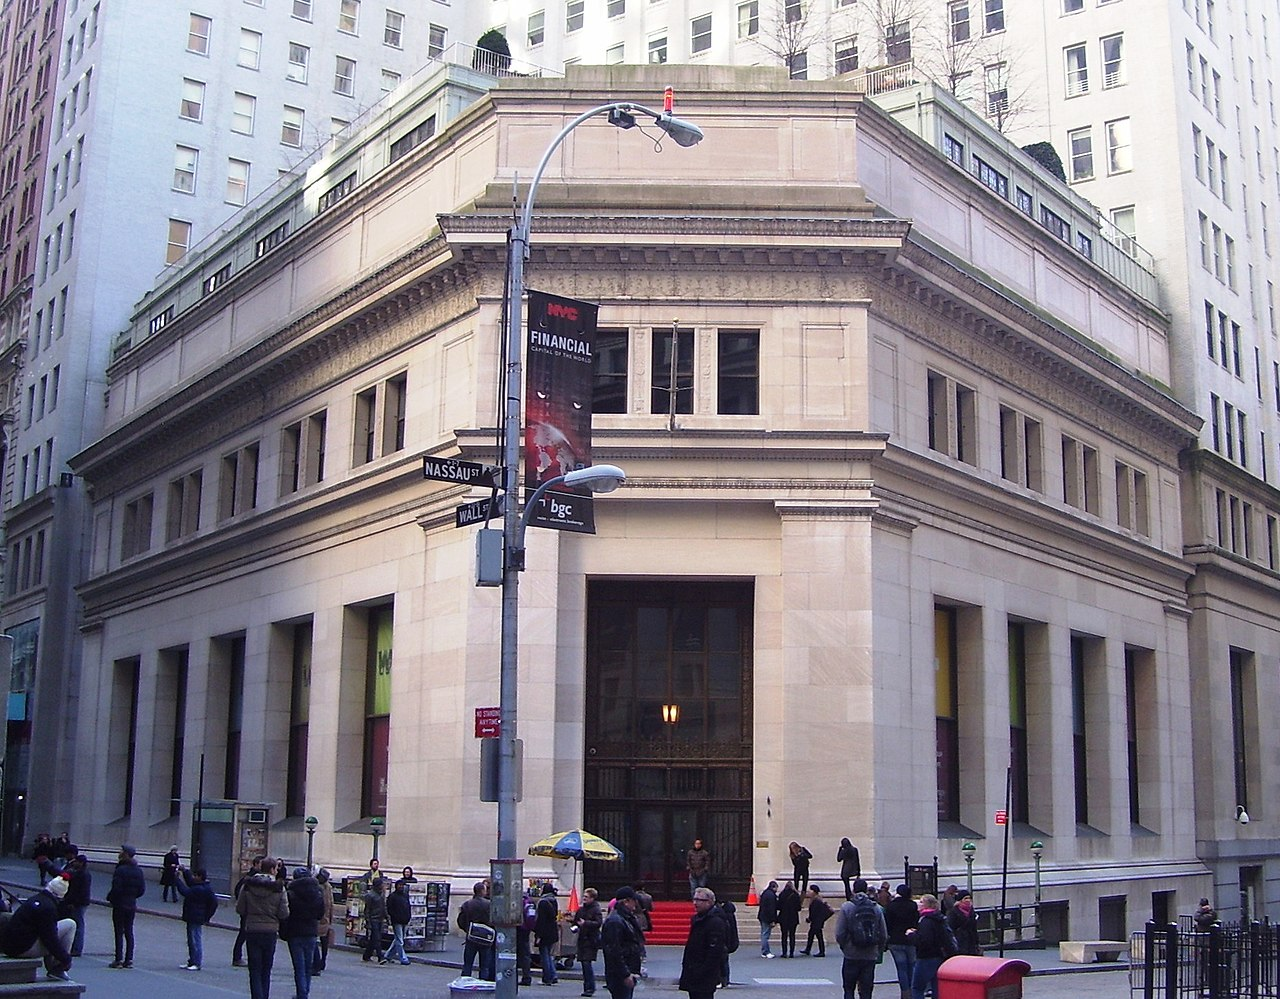
\includegraphics[height=0.40\textheight]{ch8_jpmorgan_23wall.jpg}\\[1mm]
\imgcap{Clădirea J.P. Morgan de la 23 Wall Street, New York}
\imgcredit{https://commons.wikimedia.org/wiki/File:J._P._Morgan_\%26_Company_Building_23_Wall_Street.jpg}{Foto: Beyond My Ken (2012); CC BY-SA 4.0; Wikimedia Commons}
\end{column}
\end{columns}
\end{frame}

\begin{frame}{De la RiskMetrics la Basel}
\itemsize{\footnotesize}
\begin{columns}[T]
\begin{column}{0.58\textwidth}
\begin{itemize}
    \item \textbf{BCBS} (Basel Committee on Banking Supervision, Comitetul de la Basel pentru supraveghere bancară) are sediul la \textbf{BIS}, în Basel \refBCBSh
    \begin{itemize}
        \item 1996: băncile pot calcula capitalul pentru riscul de piață cu propriile modele VaR \refBCBSa
        \item regula: VaR 1\% pe 10 zile, înmulțit cu un factor de cel puțin 3; factorul crește dacă modelul nu trece testul (backtesting) \refBCBSb
    \end{itemize}
    \item 2019: \textbf{FRTB} (Fundamental Review of the Trading Book, revizuirea fundamentală a portofoliului de tranzacționare) \refFRTB
    \begin{itemize}
        \item capitalul se calculează din ES 2,5\% în loc de VaR 1\% \refMAR; backtesting-ul numără în continuare depășirile VaR \refMARb
    \end{itemize}
\end{itemize}
\end{column}
\begin{column}{0.38\textwidth}
\centering
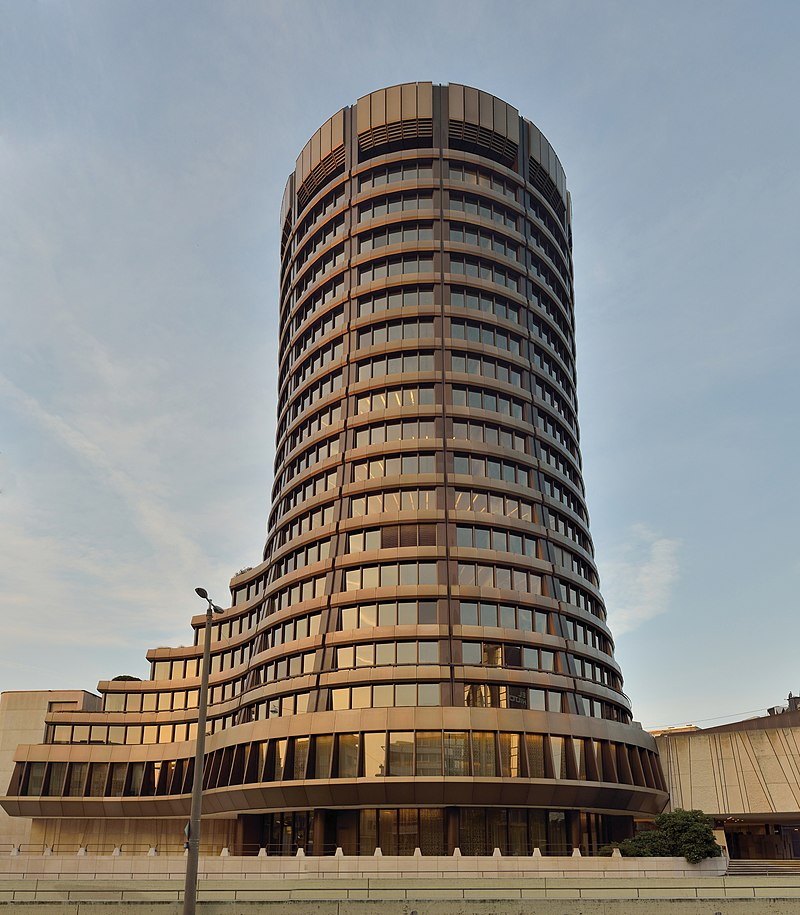
\includegraphics[height=0.42\textheight]{ch10_bis_tower_2014.jpg}\\[1mm]
\imgcap{Turnul BIS din Basel, sediul Comitetului de la Basel}
\imgcredit{https://commons.wikimedia.org/wiki/File:Basel_Committee_on_Banking_Supervision_-_BCBS.jpg}{Foto: Taxiarchos228 (2014); CC BY-SA 4.0; Wikimedia Commons}
\end{column}
\end{columns}
\end{frame}

\begin{frame}{Două furtuni: 2008 și 2020}
\itemsize{\footnotesize}
\begin{columns}[T]
\begin{column}{0.48\textwidth}
\centering
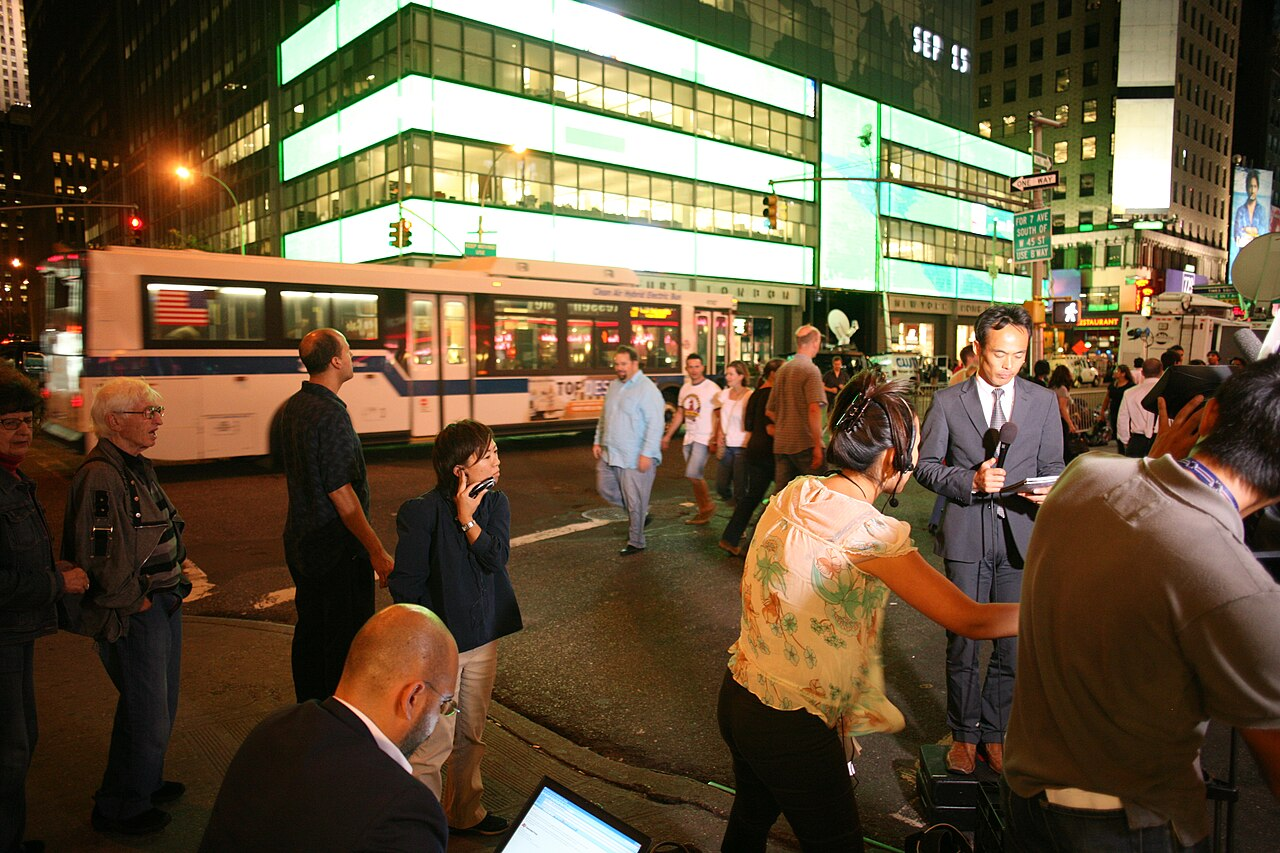
\includegraphics[height=0.30\textheight]{ch0_lehman_2008.jpg}\\[1mm]
\imgcap{Sediul Lehman Brothers, New York, 15 septembrie 2008}
\imgcredit{https://commons.wikimedia.org/wiki/File:Lehman_Brothers-NYC-20080915.jpg}{Foto: Robert Scoble (2008); CC BY 2.0; Wikimedia Commons}
\end{column}
\begin{column}{0.48\textwidth}
\centering

\includegraphics[height=0.30\textheight]{ch0_fidi_march_2020.jpg}\\[1mm]
\imgcap{Districtul financiar din New York, 25 martie 2020}
\imgcredit{https://commons.wikimedia.org/wiki/File:Subdued_FiDi_(50063555551).jpg}{Foto: Billie Grace Ward (2020); CC BY 2.0; Wikimedia Commons}
\end{column}
\end{columns}\begin{itemize}
    \item Cea mai proastă zi a S\&P 500 din 2000: $-12{,}8\%$ pe 16 martie 2020; un model Normal cu volatilitatea de selecție îi dă unei asemenea zile o probabilitate practic nulă
    \item O măsură de risc trebuie judecată în astfel de perioade: folosim 2008 și 2020 ca teste de stres în tot capitolul
\end{itemize}
\end{frame}

\begin{frame}{Recapitulare: măsurarea riscului din coadă}
\itemsize{\small}
\begin{itemize}
    \item VaR a apărut ca un rezumat zilnic al pierderii de a doua zi (RiskMetrics, 1994)
    \item Basel: VaR 1\% pentru capital (1996), ES 2,5\% pentru capital și VaR 1\% pentru backtesting (FRTB, 2019)
    \item Crizele sînt adevăratul test al unui model de risc
\end{itemize}
\end{frame}


%=============================================================================
\section{VaR și ES: definiții}
%=============================================================================

\begin{frame}{Pierderi, orizont și nivel}
\itemsize{\small}
\begin{itemize}
    \item $X$: \textbf{P\&L} (profit and loss, profitul sau pierderea) ori randamentul unei poziții pe un orizont $h$ (aici o zi, în \%)
    \begin{itemize}
        \item pierderea este $L = -X$: un număr pozitiv cînd poziția pierde bani
    \end{itemize}
    \item \textbf{Nivelul} $\alpha$ este probabilitatea cozii: $\alpha = 1\%$ sau $\alpha = 2{,}5\%$
    \begin{itemize}
        \item scriem \textbf{VaR 1\%} și \textbf{ES 2,5\%}: rezultatele proaste au probabilitatea de 1\%, respectiv 2,5\%
        \item numărul din denumire este întotdeauna probabilitatea cozii: VaR 1\% este depășit cu probabilitatea 1\%
    \end{itemize}
    \item $q_\alpha(X) = \inf\{x : P(X \le x) > \alpha\}$: \textbf{cuantila} de ordin $\alpha$ a lui $X$ (\sfmchlink{https://danpele.github.io/SFM/RO/Cursuri/capitol2_distributii_clasice_fapte_stilizate.pdf}{Capitolul 2})
    \begin{itemize}
        \item pentru o funcție de repartiție continuă $F$: $q_\alpha = F^{-1}(\alpha)$, un număr negativ pentru $\alpha$ mic
    \end{itemize}
\end{itemize}
\end{frame}

\begin{frame}{Valoarea expusă la risc (VaR)}
\itemsize{\small}
\begin{itemize}
    \item \textbf{Definiție}: $\mathrm{VaR}_\alpha(X) = -q_\alpha(X)$
    \begin{itemize}
        \item pierderea depășită cu probabilitatea $\alpha$: $P(L > \mathrm{VaR}_\alpha) \le \alpha$
        \item semnul minus face din VaR o pierdere pozitivă; un VaR de 3\% înseamnă „o pierdere de peste 3\% apare într-o zi din 100”
    \end{itemize}
    \item Ce \textbf{nu} spune VaR
    \begin{itemize}
        \item cît de mare este pierderea în zilele proaste: o pierdere de 4\% și una de 40\% dincolo de VaR dau același VaR
        \item VaR nu este pierderea maximă: prin construcție este depășit în aproximativ $\alpha$ dintre zile
    \end{itemize}
    \item În bani: o poziție cu valoarea $W$ are $\mathrm{VaR} = W \times \mathrm{VaR}(\%)/100$
\end{itemize}
\end{frame}

\begin{frame}{Expected shortfall (ES)}
\itemsize{\small}
\begin{itemize}
    \item \textbf{Definiție}: $\mathrm{ES}_\alpha(X) = -\dfrac{1}{\alpha}\displaystyle\int_0^\alpha q_u(X)\,du$: media valorilor VaR la toate nivelurile sub $\alpha$
    \begin{itemize}
        \item pentru o distribuție continuă: $\mathrm{ES}_\alpha = -E[X \mid X \le q_\alpha(X)]$, pierderea medie din cele mai proaste $\alpha$ dintre zile
        \item alte denumiri: CVaR (conditional VaR), TVaR (tail VaR), expected tail loss
    \end{itemize}
    \item Proprietăți
    \begin{itemize}
        \item $\mathrm{ES}_\alpha \ge \mathrm{VaR}_\alpha$ la același nivel $\alpha$
        \item ES privește în interiorul cozii: două distribuții cu același VaR, dar cu cozi diferite, au ES diferit
    \end{itemize}
\end{itemize}
\end{frame}

\begin{frame}{Exemplu lucrat: VaR și ES din 100 de zile}
\itemsize{\small}
\begin{itemize}
    \item O poziție are 100 de randamente zilnice; cele mai proaste cinci sînt $-6{,}1$, $-4{,}8$, $-4{,}2$, $-3{,}9$, $-3{,}5$ (în \%)
    \begin{itemize}
        \item cuantila empirică de nivel $\alpha$: al $k$-lea cel mai mic randament, $k = \lceil n\alpha \rceil$ ($\lceil\cdot\rceil$: rotunjire în sus)
    \end{itemize}
    \item \textbf{VaR 1\%}: $k = \lceil 100 \times 0{,}01 \rceil = 1$, deci $\mathrm{VaR}_{1\%} = 6{,}1\%$
    \begin{itemize}
        \item o singură observație decide VaR 1\%: cu 100 de zile, estimarea este foarte imprecisă
    \end{itemize}
    \item \textbf{ES 2,5\%}: $k = \lceil 2{,}5 \rceil = 3$; media celor mai mari trei pierderi
    \begin{itemize}
        \item $\mathrm{ES}_{2{,}5\%} = (6{,}1 + 4{,}8 + 4{,}2)/3 = 5{,}03\%$; $\mathrm{VaR}_{2{,}5\%} = 4{,}2\%$
    \end{itemize}
    \item O poziție de 1 milion de lei: VaR 1\% = 61\,000 de lei; într-o zi din o sută, pierderea este mai mare
\end{itemize}
\end{frame}

\begin{frame}{VaR 1\% și ES 2,5\% pentru S\&P 500}
\itemsize{\footnotesize}
\begin{center}
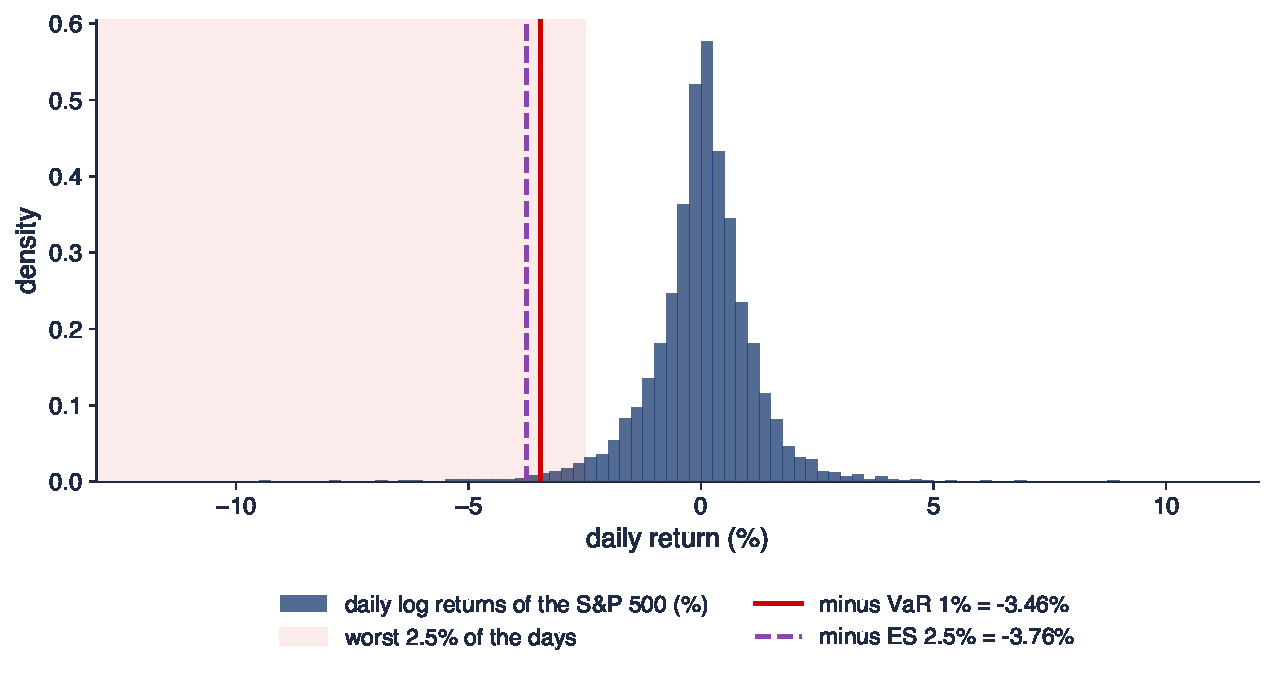
\includegraphics[width=0.97\textwidth,height=0.50\textheight,keepaspectratio]{sfm_ch10_var_es_def.pdf}
\end{center}
\vspace{-0.25cm}
\begin{itemize}
    \item Randamente logaritmice zilnice din 2000 (6\,714 zile); estimări istorice: VaR 1\% $= 3{,}46\%$, VaR 2,5\% $= 2{,}51\%$, ES 2,5\% $= 3{,}76\%$
    \item Interpretare: ES 2,5\% face media întregii cozi hașurate, inclusiv a zilelor extreme din 2008 și 2020; VaR 1\% este un singur punct din această coadă
    \item Pentru o poziție de 1 milion de lei în indice: VaR 1\% circa 34\,552 lei, ES 2,5\% circa 37\,613 lei
\end{itemize}
\sfmquantlet{Ch_10}{SFM_ch10_var_methods}
\end{frame}

\begin{frame}{Distribuția Normală: formule explicite}
\itemsize{\footnotesize}
\begin{itemize}
    \item $X \sim N(\mu, \sigma^2)$, $z_\alpha = \Phi^{-1}(\alpha)$ ($\Phi$, $\varphi$: funcția de repartiție și densitatea lui $N(0,1)$)
    \begin{itemize}
        \item $\mathrm{VaR}_\alpha = -(\mu + \sigma z_\alpha)$, \quad $\mathrm{ES}_\alpha = -\mu + \sigma\,\dfrac{\varphi(z_\alpha)}{\alpha}$
        \item derivare: $E[Z \mid Z \le z] = -\varphi(z)/\Phi(z)$, deoarece $\varphi'(z) = -z\varphi(z)$
    \end{itemize}
    \item Valori: $z_{0{,}01} = -2{,}326$; $z_{0{,}025} = -1{,}960$, $\varphi(z_{0{,}025}) = 0{,}0584$, $\varphi(z_{0{,}025})/0{,}025 = 2{,}338$
    \begin{itemize}
        \item ES 2,5\% / VaR 1\% $= 2{,}338/2{,}326 = 1{,}005$ (cu $\mu = 0$): pentru randamente Normale, cele două măsuri sînt aproape egale
        \item de aceea ES 2,5\% a înlocuit VaR 1\% în Basel: aceeași mărime pentru date Normale, mai mare pentru cozi groase
    \end{itemize}
\end{itemize}
\end{frame}

\begin{frame}{Exemplu lucrat: VaR și ES Normale pentru S\&P 500}
\itemsize{\small}
\begin{itemize}
    \item Momentele de selecție ale randamentelor zilnice din 2000: $\hat\mu = 0{,}025$, $\hat\sigma = 1{,}21$ (în \%)
    \begin{itemize}
        \item VaR 1\% $= -(0{,}025 - 2{,}326 \times 1{,}21) = -0{,}025 + 2{,}822 = 2{,}80\%$
        \item ES 2,5\% $= -0{,}025 + 2{,}338 \times 1{,}21 = -0{,}025 + 2{,}836 = 2{,}81\%$
    \end{itemize}
    \item Comparăm cu datele (simulare istorică): VaR 1\% $= 3{,}46\%$, ES 2,5\% $= 3{,}76\%$
    \begin{itemize}
        \item VaR 1\% Normal este prea mic cu 19\%: coada distribuției Normale este prea subțire (\sfmchlink{https://danpele.github.io/SFM/RO/Cursuri/capitol2_distributii_clasice_fapte_stilizate.pdf}{Capitolul 2})
        \item ES 2,5\% Normal este și mai departe de date: ignoră zilele extreme
    \end{itemize}
    \item Interpretare: doi parametri nu pot descrie coada; metodele următoare schimbă fie distribuția, fie datele folosite
\end{itemize}
\end{frame}

\begin{frame}{Distribuția Student-t: formule explicite}
\itemsize{\footnotesize}
\begin{itemize}
    \item $X = m + s\,T$, $T \sim t_\nu$ (poziția $m$, scala $s$, $\nu$ grade de libertate, \sfmchlink{https://danpele.github.io/SFM/RO/Cursuri/capitol2_distributii_clasice_fapte_stilizate.pdf}{Capitolul 2}); $t_\alpha = t_\nu^{-1}(\alpha)$, $f_\nu$ densitatea lui $t_\nu$
    \begin{itemize}
        \item $\mathrm{VaR}_\alpha = -(m + s\,t_\alpha)$, \quad $\mathrm{ES}_\alpha = -m + s\,\dfrac{f_\nu(t_\alpha)}{\alpha}\,\dfrac{\nu + t_\alpha^2}{\nu - 1}$ (pentru $\nu > 1$)
        \item varianța este $s^2\nu/(\nu - 2)$: o t \textbf{standardizată} (varianța 1) are $s = \sqrt{(\nu - 2)/\nu}$
    \end{itemize}
    \item \textbf{Exemplu lucrat}: S\&P 500, verosimilitate maximă: $\hat m = 0{,}068$, $\hat s = 0{,}703$, $\hat\nu = 2{,}67$
    \begin{itemize}
        \item $t_{0{,}01} = -5{,}023$: VaR 1\% $= -(0{,}068 + 0{,}703 \times (-5{,}023)) = 3{,}46\%$
        \item factorul ES $5{,}720$: ES 2,5\% $= -0{,}068 + 0{,}703 \times 5{,}720 = 3{,}95\%$
    \end{itemize}
    \item Interpretare: cu $\nu < 3$, coada estimată este foarte groasă: VaR 1\% se potrivește cu datele, ES 2,5\% este peste valoarea istorică de $3{,}76\%$
\end{itemize}
\end{frame}

\begin{frame}{De la o zi la zece zile}
\itemsize{\footnotesize}
\begin{itemize}
    \item \textbf{Regula rădăcinii pătrate a timpului}: $\mathrm{VaR}^{(h)} \approx \sqrt{h}\,\mathrm{VaR}^{(1)}$
    \begin{itemize}
        \item exactă pentru randamente Normale i.i.d.\ cu media 0: randamentul pe $h$ zile are abaterea standard $\sigma\sqrt{h}$
        \item Basel 1996: VaR pe 10 zile, de obicei scalat de la o zi cu $\sqrt{10} = 3{,}162$
    \end{itemize}
    \item S\&P 500, simulare istorică
    \begin{itemize}
        \item o zi: 3{,}46\%; scalat: $3{,}162 \times 3{,}46 = 10{,}93\%$
        \item VaR 1\% al randamentelor pe 10 zile suprapuse: 10{,}37\%
    \end{itemize}
    \item De ce regula nu funcționează în general
    \begin{itemize}
        \item cozi groase: suma a 10 randamente cu cozi groase este mai aproape de Normală (CLT, teorema limită centrală), deci raportul cuantilelor este sub $\sqrt{10}$
        \item volatility clustering: după o zi liniștită, riscul pe 10 zile este mai mare decît $\sqrt{10}$ ori riscul de azi, după o furtună mai mic (\sfmchlink{https://danpele.github.io/SFM/RO/Cursuri/capitol9_modele_arch_garch.pdf}{Capitolul 9})
    \end{itemize}
\end{itemize}
\end{frame}

\begin{frame}{Recapitulare: definițiile VaR și ES}
\itemsize{\small}
\begin{itemize}
    \item $\mathrm{VaR}_\alpha = -q_\alpha$: pierderea depășită cu probabilitatea $\alpha$; $\mathrm{ES}_\alpha$: pierderea medie dincolo de ea
    \item Distribuția Normală: ES 2,5\% $\approx$ VaR 1\%; cozile groase fac ES 2,5\% mai mare
    \item Scalarea la 10 zile cu $\sqrt{10}$ este o convenție, nu o lege
\end{itemize}
\end{frame}


%=============================================================================
\section{Măsuri de risc coerente}
%=============================================================================

\begin{frame}{1999: patru axiome pentru o măsură de risc}
\itemsize{\footnotesize}
\begin{columns}[T]
\begin{column}{0.64\textwidth}
\begin{itemize}
    \item \refArtzner: o măsură de risc $\rho$ asociază unei pierderi $L$ capitalul care o face acceptabilă; $\rho$ este \textbf{coerentă} dacă
    \begin{itemize}
        \item \textbf{monotonie}: $L_1 \le L_2$ întotdeauna $\Rightarrow \rho(L_1) \le \rho(L_2)$
        \item \textbf{invarianță la translație}: $\rho(L + c) = \rho(L) + c$ pentru o sumă sigură $c$
        \item \textbf{omogenitate pozitivă}: $\rho(\lambda L) = \lambda\rho(L)$, $\lambda > 0$
        \item \textbf{subaditivitate}: $\rho(L_1 + L_2) \le \rho(L_1) + \rho(L_2)$
    \end{itemize}
    \item Subaditivitatea: diversificarea nu adaugă niciodată risc; o bancă poate aduna capitalul diviziilor ca margine superioară
\end{itemize}
\end{column}
\begin{column}{0.32\textwidth}
\centering

\includegraphics[height=0.40\textheight]{ch10_delbaen_1997.jpg}\\[1mm]
\imgcap{Freddy Delbaen, coautor al axiomelor (1997)}
\imgcredit{https://commons.wikimedia.org/wiki/File:ETH-BIB-Delbaen,_Freddy_(1946-)-Portr_16468.tif}{Foto: ETH-Bibliothek Zürich, Bildarchiv (1997); CC BY-SA 4.0; Wikimedia Commons}
\end{column}
\end{columns}
\end{frame}

\begin{frame}{Contraexemplu: două obligațiuni, pas cu pas}
\itemsize{\footnotesize}
\begin{itemize}
    \item Două obligațiuni independente; fiecare pierde 100 cu probabilitatea 4\% (neplată) și 0 în rest; nivelul $\alpha = 5\%$
    \begin{itemize}
        \item o obligațiune: $P(L > 0) = 4\% \le 5\%$, deci $\mathrm{VaR}_{5\%} = 0$ pentru fiecare
    \end{itemize}
    \item Ambele obligațiuni: $P(L = 200) = 0{,}16\%$, $P(L = 100) = 7{,}68\%$, deci $P(L > 0) = 7{,}84\% > 5\%$
    \begin{itemize}
        \item $\mathrm{VaR}_{5\%}(L_1 + L_2) = 100 > 0 + 0$: VaR \textbf{penalizează} diversificarea
    \end{itemize}
    \item ES 5\% (media celor mai proaste 5\% dintre rezultate)
    \begin{itemize}
        \item o obligațiune: $(4\% \times 100 + 1\% \times 0)/5\% = 80$
        \item ambele: $(0{,}16\% \times 200 + (5 - 0{,}16)\% \times 100)/5\% = 103{,}2 \le 80 + 80$: subaditiv
    \end{itemize}
\end{itemize}
\end{frame}

\begin{frame}{ES este coerent; VaR doar uneori}
\itemsize{\small}
\begin{itemize}
    \item \textbf{ES} satisface toate cele patru axiome \refAT
    \begin{itemize}
        \item motivul: ES este o medie a cuantilelor pe coadă, iar media respectă sumele
    \end{itemize}
    \item \textbf{VaR} le satisface pe primele trei; subaditivitatea poate să nu fie îndeplinită
    \begin{itemize}
        \item nu este îndeplinită pentru pierderi discrete (credit, obligațiunile de mai sus) și pentru cozi extrem de groase (indicele de coadă sub 1, \sfmchlink{https://danpele.github.io/SFM/RO/Cursuri/capitol5_cozi_groase_evt.pdf}{Capitolul 5})
        \item este îndeplinită pentru distribuțiile eliptice (Normală, Student-t) și, în practică, pentru majoritatea randamentelor de acțiuni \refDJSS
    \end{itemize}
    \item ES are nevoie de o medie finită a pierderilor; VaR există întotdeauna
\end{itemize}
\end{frame}

\begin{frame}{Elicitabilitatea: evaluarea prognozelor}
\itemsize{\small}
\begin{itemize}
    \item O statistică este \textbf{elicitabilă} dacă o funcție de pierdere (de scor) este minimizată, în medie, de valoarea ei adevărată \refGneiting
    \begin{itemize}
        \item media: eroarea pătratică; mediana: eroarea absolută
    \end{itemize}
    \item \textbf{VaR este elicitabil}: pierderea cuantilă (pinball) $S(v, x) = (\alpha - \mathbf{1}\{x < -v\})(x + v)$
    \begin{itemize}
        \item două modele VaR pot fi comparate prin media pierderii cuantile
    \end{itemize}
    \item \textbf{ES singur nu este elicitabil} \refGneiting; perechea (VaR, ES) este elicitabilă \refFZ
    \begin{itemize}
        \item consecința: prognozele ES se testează împreună cu prognozele VaR (secțiunea 7)
    \end{itemize}
\end{itemize}
\end{frame}

\begin{frame}{Recapitulare: măsuri de risc coerente}
\itemsize{\small}
\begin{itemize}
    \item Coerența: monotonie, invarianță la translație, omogenitate pozitivă, subaditivitate
    \item ES este coerent; VaR poate penaliza diversificarea (cele două obligațiuni)
    \item VaR este elicitabil, ES doar împreună cu VaR
\end{itemize}
\end{frame}


%=============================================================================
\section{Estimarea VaR și ES}
%=============================================================================

\begin{frame}{Cinci metode necondiționate, pe scurt}
\itemsize{\footnotesize}
\begin{center}
\footnotesize
\begin{tabular}{>{\raggedright\arraybackslash}p{2.3cm}>{\raggedright\arraybackslash}p{4.0cm}>{\raggedright\arraybackslash}p{4.6cm}}
\toprule
\textbf{Metoda} & \textbf{Ipoteza} & \textbf{Punctul slab} \\
\midrule
simulare istorică (HS) & fereastra trecută este un eșantion din ziua de mîine & puține puncte în coadă; nimic dincolo de cea mai proastă zi \\
Normală & randamentele sînt Normale & cozi mult prea subțiri \\
Student-t & randamentele urmează o distribuție Student-t & o singură formă pentru ambele cozi \\
Cornish--Fisher & cuantila Normală corectată prin asimetrie și boltire & nu mai funcționează pentru boltire mare \\
EVT (POT) & distribuția GPD peste un prag ridicat (\sfmchlink{https://danpele.github.io/SFM/RO/Cursuri/capitol5_cozi_groase_evt.pdf}{Capitolul 5}) & alegerea pragului \\
\bottomrule
\end{tabular}
\end{center}
\begin{itemize}
    \item „Necondiționat”: același VaR în fiecare zi a ferestrei; metodele condiționate (secțiunea 5) folosesc volatilitatea de azi
    \item Toate metodele: randamente logaritmice zilnice în \% (\sfmchlink{https://danpele.github.io/SFM/RO/Cursuri/capitol1_date_randamente_indicatori.pdf}{Capitolul 1}), VaR și ES ca pierderi pozitive
\end{itemize}
\end{frame}

\begin{frame}{Simularea istorică}
\itemsize{\small}
\begin{itemize}
    \item \textbf{Algoritmul}: luăm ultimele $n$ randamente $r_{t-n+1}, \dots, r_t$ și le ordonăm: $r_{(1)} \le \dots \le r_{(n)}$
    \begin{itemize}
        \item $\widehat{\mathrm{VaR}}_\alpha = -r_{(k)}$, $k = \lceil n\alpha \rceil$; \quad $\widehat{\mathrm{ES}}_\alpha = -\frac{1}{k}\sum_{i=1}^{k} r_{(i)}$
        \item nu presupunem nicio distribuție: distribuția empirică a ferestrei este prognoza
    \end{itemize}
    \item Portat din Quantlet-ul SFE VaRest
\end{itemize}
\end{frame}

\begin{frame}{Exemplu lucrat: simularea istorică pentru S\&P 500}
\itemsize{\footnotesize}
\begin{itemize}
    \item S\&P 500 din 2000: $n = 6\,714$
    \begin{itemize}
        \item VaR 1\%: $k = \lceil 67{,}14 \rceil = 68$, a 68-a cea mai proastă zi: $3{,}46\%$
        \item ES 2,5\%: media celor mai proaste $\lceil 167{,}85 \rceil = 168$ zile: $3{,}76\%$
    \end{itemize}
    \item Fereastra $n$ este un compromis
    \begin{itemize}
        \item scurtă (250 de zile): reacționează, dar VaR 1\% se bazează pe 3 observații; lungă (toate datele): stabilă, dar insensibilă la volatilitatea de azi
        \item \textbf{efectul de fantomă}: o zi de crah schimbă VaR cînd intră în fereastră și din nou, brusc, după $n$ zile, cînd iese din ea
    \end{itemize}
\end{itemize}
\end{frame}

\begin{frame}{Precizia unui VaR istoric}
\itemsize{\footnotesize}
\begin{itemize}
    \item O estimare VaR este o statistică: are o eroare de eșantionare; o măsurăm prin bootstrap (\sfmchlink{https://danpele.github.io/SFM/RO/Cursuri/capitol2_distributii_clasice_fapte_stilizate.pdf}{Capitolul 2})
    \begin{itemize}
        \item reeșantionăm cele $n$ randamente cu întoarcere de 2000 de ori, recalculăm VaR și ES și citim cuantilele de 2,5\% și 97,5\%
    \end{itemize}
    \item S\&P 500, toate cele 6\,714 zile: VaR 1\% $= 3{,}46\%$, intervalul de 95\% [3{,}18; 3{,}66]; ES 2,5\% $= 3{,}76\%$, [3{,}46; 4{,}07]
    \begin{itemize}
        \item ultimele 500 de zile: VaR 1\% $= 2{,}75\%$, [1{,}99; 4{,}96]; ES 2,5\% $= 2{,}94\%$, [2{,}14; 3{,}82]
    \end{itemize}
    \item Cu doi ani de date, intervalul pentru VaR 1\% are o lățime de peste 2 puncte procentuale: VaR 1\% se bazează pe 5 observații
    \item Interpretare: diferențele dintre metode mai mici decît intervalul bootstrap nu dovedesc că o metodă este mai bună
\end{itemize}\sfmquantlet{Ch_10}{SFM_ch10_var_methods}
\end{frame}

\begin{frame}{Dezvoltarea Cornish--Fisher}
\itemsize{\footnotesize}
\begin{itemize}
    \item \refCF: corectăm cuantila Normală $z = z_\alpha$ cu asimetria $S$ și excesul de boltire $K$ (coeficientul de boltire minus 3)
    \begin{itemize}
        \item $z_{CF} = z + \dfrac{(z^2 - 1)S}{6} + \dfrac{(z^3 - 3z)K}{24} - \dfrac{(2z^3 - 5z)S^2}{36}$, \quad $\mathrm{VaR}_\alpha = -(\mu + \sigma z_{CF})$
        \item $S$ negativ și $K$ pozitiv împing cuantila mai departe în coada stîngă
    \end{itemize}
    \item S\&P 500: $S = -0{,}35$, $K = 10{,}7$, $z_{0{,}01} = -2{,}326$
    \begin{itemize}
        \item $z_{CF} = -5{,}03$, deci VaR 1\% $= 6{,}08\%$, față de valoarea istorică de $3{,}46\%$
    \end{itemize}
    \item Interpretare: dezvoltarea este o corecție mică în jurul distribuției Normale; cu un exces de boltire de peste 10, ea depășește mult valoarea corectă
    \begin{itemize}
        \item o folosim doar cînd $|S|$ și $K$ sînt moderate (de exemplu, pentru randamente lunare sau portofolii diversificate)
    \end{itemize}
\end{itemize}
\end{frame}

\begin{frame}{EVT: peaks over threshold (\sfmchlinkt{https://danpele.github.io/SFM/RO/Cursuri/capitol5_cozi_groase_evt.pdf}{Capitolul 5})}
\itemsize{\footnotesize}
\begin{itemize}
    \item Pierderile $L = -r$; pragul $u$ = cuantila de 90\% a pierderilor \refMF; excesele $L - u$ peste $u$ urmează o distribuție GPD (Pareto generalizată) cu forma $\xi$ și scala $\beta$
    \begin{itemize}
        \item $\mathrm{VaR}_\alpha = u + \dfrac{\beta}{\xi}\Big[\Big(\dfrac{n\alpha}{N_u}\Big)^{-\xi} - 1\Big]$, \quad $\mathrm{ES}_\alpha = \dfrac{\mathrm{VaR}_\alpha + \beta - \xi u}{1 - \xi}$ ($N_u$: numărul de excese)
    \end{itemize}
    \item S\&P 500: $u = 1{,}26\%$, $N_u = 672$ (10{,}0\% dintre zile), $\hat\xi = 0{,}164$, $\hat\beta = 0{,}820$
    \begin{itemize}
        \item VaR 1\%: $n\alpha/N_u = 0{,}0999$, $0{,}0999^{-\hat\xi} = 1{,}461$; $1{,}26 + 4{,}988 \times (1{,}461 - 1) = 3{,}56\%$
        \item ES 2,5\% $= 3{,}77\%$; $\hat\xi > 0$: o coadă groasă (de tip Pareto)
    \end{itemize}
    \item EVT netezește coada și extrapolează dincolo de cea mai proastă zi observată: util pentru VaR 0,1\% și pentru testele de stres
\end{itemize}
\end{frame}

\begin{frame}{VaR pentru diferite probabilități ale cozii}
\itemsize{\footnotesize}
\begin{center}
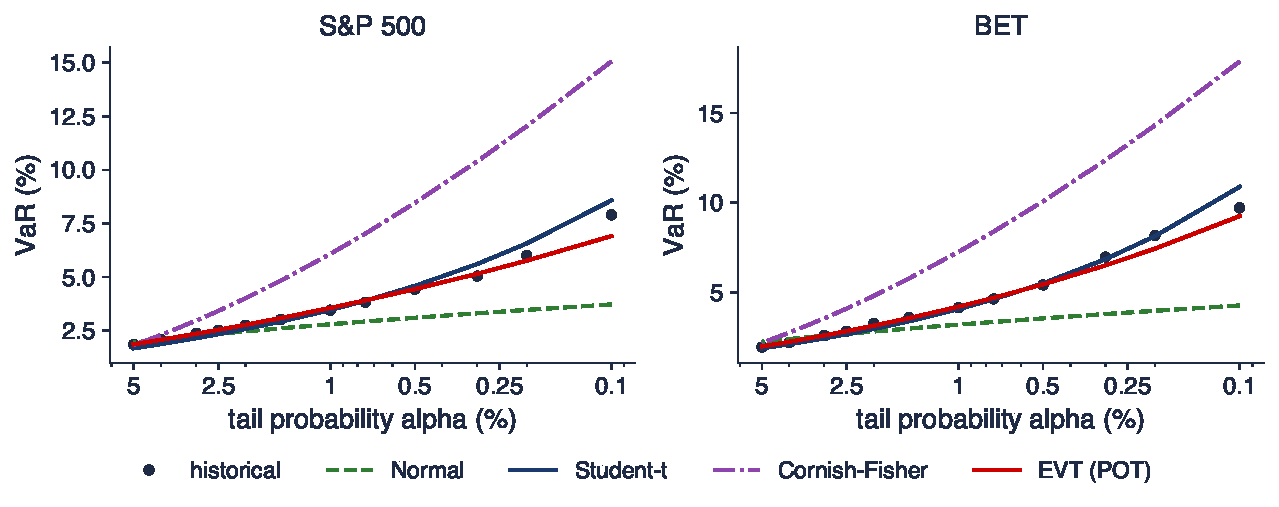
\includegraphics[width=0.97\textwidth,height=0.52\textheight,keepaspectratio]{sfm_ch10_var_curves.pdf}
\end{center}
\vspace{-0.25cm}
\begin{itemize}
    \item Fiecare linie: $\mathrm{VaR}_\alpha$ al unei metode pentru $\alpha$ de la 5\% la 0,1\%; punctele: simularea istorică
    \item Interpretare: la 5\% toate metodele sînt de acord; la 1\% distribuția Normală dă valori prea mici; la 0,1\% Student-t și EVT rămîn aproape de date, iar Cornish--Fisher crește exploziv
\end{itemize}
\sfmquantlet{Ch_10}{SFM_ch10_var_methods}
\end{frame}

\begin{frame}{VaR 1\% pe metode, pentru șase serii}
\itemsize{\footnotesize}
\begin{center}
\footnotesize
\begin{tabular}{lrrrrrrr}
\toprule
& HS & Normală & Student-t & Cornish--Fisher & EVT & $K$ & $\hat\xi$ \\
\midrule
S\&P 500 & $3{,}46$ & $2{,}80$ & $3{,}46$ & $6{,}08$ & $3{,}56$ & ${10{,}7}$ & $0{,}16$ \\
DAX & $4{,}20$ & $3{,}26$ & $3{,}96$ & $5{,}42$ & $4{,}05$ & ${6{,}1}$ & $0{,}12$ \\
BET & $4{,}14$ & $3{,}19$ & $4{,}06$ & $7{,}25$ & $4{,}19$ & ${11{,}1}$ & $0{,}23$ \\
Bitcoin & $10{,}54$ & $7{,}99$ & $11{,}06$ & $18{,}89$ & $10{,}38$ & ${12{,}0}$ & $0{,}12$ \\
TLV & $5{,}11$ & $4{,}01$ & $4{,}63$ & $10{,}19$ & $4{,}90$ & ${13{,}5}$ & $0{,}26$ \\
SNP & $4{,}29$ & $3{,}70$ & $4{,}26$ & $7{,}55$ & $4{,}38$ & ${8{,}9}$ & $0{,}22$ \\
\bottomrule
\end{tabular}
\end{center}
\begin{itemize}
    \item Eșantioanele complete (S\&P 500, DAX, BET din 2000; Bitcoin din 2014; TLV și SNP din 2010), în \%; $K$: excesul de boltire
    \item HS, Student-t și EVT diferă cu cel mult 0{,}7 puncte procentuale; VaR-ul Normal este peste tot prea mic cu 14--24\%
    \item Cornish--Fisher dă de 1{,}3 pînă la 2{,}0 ori VaR-ul istoric: cu $K$ între 6 și 14, dezvoltarea este în afara domeniului ei de valabilitate
\end{itemize}\sfmquantlet{Ch_10}{SFM_ch10_var_methods}
\end{frame}

\begin{frame}{ES 2,5\% pe metode, pentru șase serii}
\itemsize{\footnotesize}
\begin{center}
\footnotesize
\begin{tabular}{lrrrrrrr}
\toprule
& HS & Normală & Student-t & Cornish--Fisher & EVT & $K$ & $\hat\xi$ \\
\midrule
S\&P 500 & $3{,}76$ & $2{,}81$ & $3{,}95$ & $6{,}65$ & $3{,}77$ & ${10{,}7}$ & $0{,}16$ \\
DAX & $4{,}26$ & $3{,}27$ & $4{,}37$ & $5{,}81$ & $4{,}24$ & ${6{,}1}$ & $0{,}12$ \\
BET & $4{,}57$ & $3{,}21$ & $4{,}76$ & $7{,}93$ & $4{,}57$ & ${11{,}1}$ & $0{,}23$ \\
Bitcoin & $10{,}84$ & $8{,}03$ & $13{,}37$ & $20{,}69$ & $10{,}90$ & ${12{,}0}$ & $0{,}12$ \\
TLV & $5{,}37$ & $4{,}03$ & $5{,}03$ & $11{,}20$ & $5{,}35$ & ${13{,}5}$ & $0{,}26$ \\
SNP & $4{,}70$ & $3{,}72$ & $4{,}57$ & $8{,}18$ & $4{,}71$ & ${8{,}9}$ & $0{,}22$ \\
\bottomrule
\end{tabular}
\end{center}
\begin{itemize}
    \item Distribuția Normală: ES 2,5\% este egal cu VaR 1\%; datele: ES 2,5\% istoric este cu 1{,}5--10{,}5\% peste VaR 1\% istoric
    \item Pentru S\&P 500, DAX, BET și Bitcoin, Student-t dă cel mai mare ES dintre metodele rezonabile (Bitcoin: $13{,}37\%$ față de $10{,}84\%$): cu $\hat\nu < 3$, coada ei este mai groasă decît cea a datelor de dincolo de prag
    \item Interpretare: EVT și HS sînt de acord la 2,5\%; metoda contează mai mult pentru ES decît pentru VaR, deoarece ES depinde de întreaga coadă
\end{itemize}\sfmquantlet{Ch_10}{SFM_ch10_var_methods}
\end{frame}

\begin{frame}{Recapitulare: estimarea VaR și ES}
\itemsize{\small}
\begin{itemize}
    \item HS: fereastra ordonată; Normală și Student-t: formule explicite; Cornish--Fisher: corecție prin momente; EVT: coada GPD
    \item Pe date zilnice: distribuția Normală dă valori prea mici, Cornish--Fisher prea mari; HS, Student-t și EVT sînt apropiate la 1\%
    \item Toate cele cinci metode ignoră volatilitatea de azi
\end{itemize}
\end{frame}


%=============================================================================
\section{VaR condiționat: GARCH și simularea istorică filtrată}
%=============================================================================

\begin{frame}{Rolul volatilității de azi}
\itemsize{\footnotesize}
\begin{itemize}
    \item Volatility clustering (\sfmchlink{https://danpele.github.io/SFM/RO/Cursuri/capitol8_estimatori_volatilitate.pdf}{Capitolele 8} și \sfmchlink{https://danpele.github.io/SFM/RO/Cursuri/capitol9_modele_arch_garch.pdf}{9}): după o zi liniștită urmează zile liniștite, după o furtună urmează furtuni
    \begin{itemize}
        \item un VaR necondiționat este prea mare în anii liniștiți și prea mic la începutul unei crize
    \end{itemize}
    \item Modelul condiționat: $r_{t+1} = \mu + \sigma_{t+1}z_{t+1}$, $z$ i.i.d.\ cu media 0 și varianța 1
    \begin{itemize}
        \item $\mathrm{VaR}_{t+1} = -(\mu + \sigma_{t+1}\,q_\alpha(z))$, \quad $\mathrm{ES}_{t+1} = -\mu + \sigma_{t+1}\,\mathrm{ES}_\alpha(z)$
        \item două ingrediente: prognoza volatilității $\sigma_{t+1}$ și distribuția lui $z$
    \end{itemize}
    \item Două variante pentru distribuția lui $z$
    \begin{itemize}
        \item \textbf{GARCH-t}: Student-t standardizată, cu $\nu$ estimat împreună cu GARCH(1,1) \refBoll
        \item \textbf{FHS} (filtered historical simulation, simularea istorică filtrată): distribuția empirică a reziduurilor standardizate $\hat z_t = (r_t - \hat\mu)/\hat\sigma_t$ \refHW; \refBGV
    \end{itemize}
\end{itemize}
\end{frame}

\begin{frame}{Exemplu lucrat: S\&P 500 la 18 septembrie 2026}
\itemsize{\footnotesize}
\begin{itemize}
    \item GARCH(1,1)-t pe toate datele: $\hat\mu = 0{,}079$, $\hat\alpha = 0{,}123$, $\hat\beta = 0{,}872$, $\hat\nu = 6{,}26$; prognoza pentru ziua următoare $\sigma_{t+1} = 0{,}714\%$
    \item \textbf{GARCH-t}: $q_{0{,}01}(z) = t_\nu^{-1}(0{,}01)\sqrt{(\nu - 2)/\nu} = -2{,}557$; $\mathrm{ES}_{2{,}5\%}(z) = 2{,}644$
    \begin{itemize}
        \item VaR 1\% $= -(0{,}079 + 0{,}714 \times (-2{,}557)) = 1{,}75\%$; ES 2,5\% $= -0{,}079 + 0{,}714 \times 2{,}644 = 1{,}81\%$
    \end{itemize}
    \item \textbf{FHS}: cuantila de 1\% a celor 6\,714 reziduuri standardizate este $-2{,}787$; ES 2,5\% al lor este $2{,}952$
    \begin{itemize}
        \item VaR 1\% $= -(0{,}079 + 0{,}714 \times (-2{,}787)) = 1{,}91\%$; ES 2,5\% $= 2{,}03\%$
    \end{itemize}
    \item Interpretare: o piață liniștită: VaR 1\% condiționat este cam jumătate din valoarea necondiționată de $3{,}46\%$; reziduurile standardizate au o coadă stîngă mai groasă decît t estimată
\end{itemize}\sfmquantlet{Ch_10}{SFM_ch10_conditional_var}
\end{frame}

\begin{frame}{VaR și ES pentru ziua următoare, pe șase serii}
\itemsize{\footnotesize}
\begin{center}
\footnotesize
\begin{tabular}{lrrrrrrr}
\toprule
& \multicolumn{3}{c}{VaR 1\%} & \multicolumn{3}{c}{ES 2,5\%} & \\ & HS (tot) & GARCH-t & FHS & HS (tot) & GARCH-t & FHS & $\sigma_{t+1}$ \\
\midrule
S\&P 500 & $3{,}46$ & $1{,}75$ & $1{,}91$ & $3{,}76$ & $1{,}81$ & $2{,}03$ & $0{,}714$ \\
DAX & $4{,}20$ & $2{,}31$ & $2{,}48$ & $4{,}26$ & $2{,}38$ & $2{,}55$ & $0{,}945$ \\
BET & $4{,}14$ & $4{,}51$ & $4{,}81$ & $4{,}57$ & $4{,}72$ & $5{,}04$ & $1{,}763$ \\
Bitcoin & $10{,}54$ & $7{,}37$ & $7{,}99$ & $10{,}84$ & $8{,}11$ & $8{,}57$ & $2{,}829$ \\
TLV & $5{,}11$ & $7{,}18$ & $7{,}33$ & $5{,}37$ & $7{,}53$ & $8{,}00$ & $2{,}791$ \\
SNP & $4{,}29$ & $5{,}06$ & $5{,}39$ & $4{,}70$ & $5{,}31$ & $5{,}65$ & $1{,}966$ \\
\bottomrule
\end{tabular}
\end{center}
\begin{itemize}
    \item Prognoze pentru ziua de după 18 septembrie 2026, în \%; HS (tot): valorile istorice necondiționate din secțiunea precedentă
    \item S\&P 500, DAX, Bitcoin: perioadă liniștită, valorile condiționate sînt sub cele necondiționate
    \item Interpretare: BET, TLV și SNP: volatilitatea curentă este mare, deci VaR condiționat este peste VaR istoric de lungă durată; aceeași metodă transmite mesaje opuse pe piețe diferite
\end{itemize}\sfmquantlet{Ch_10}{SFM_ch10_conditional_var}
\end{frame}

\begin{frame}{Prognoze pe fereastră mobilă: designul}
\itemsize{\small}
\begin{itemize}
    \item \textbf{În afara eșantionului}: prognoza pentru ziua $t$ folosește doar date pînă în ziua $t-1$
    \begin{itemize}
        \item S\&P 500, DAX, BET: fiecare zi din ianuarie 2005 (inclusiv 2008); Bitcoin: din ianuarie 2017
    \end{itemize}
    \item Patru metode
    \begin{itemize}
        \item \textbf{HS} și \textbf{Normală}: ultimele 500 de zile (circa doi ani)
        \item \textbf{GARCH-t} și \textbf{FHS}: GARCH(1,1)-t reestimat la fiecare 250 de zile pe toate datele trecute; $\sigma_t$ actualizat zilnic
    \end{itemize}
    \item În fiecare zi: VaR 1\% (pentru backtesting), VaR 2,5\% și ES 2,5\% (pentru backtesting-ul ES)
    \item Portat din SFEVaRtimeplot și SFEVaRbank
\end{itemize}\sfmquantlet{Ch_10}{SFM_ch10_conditional_var}
\end{frame}

\begin{frame}{VaR 1\% în 2008 și în 2020}
\itemsize{\footnotesize}
\begin{center}
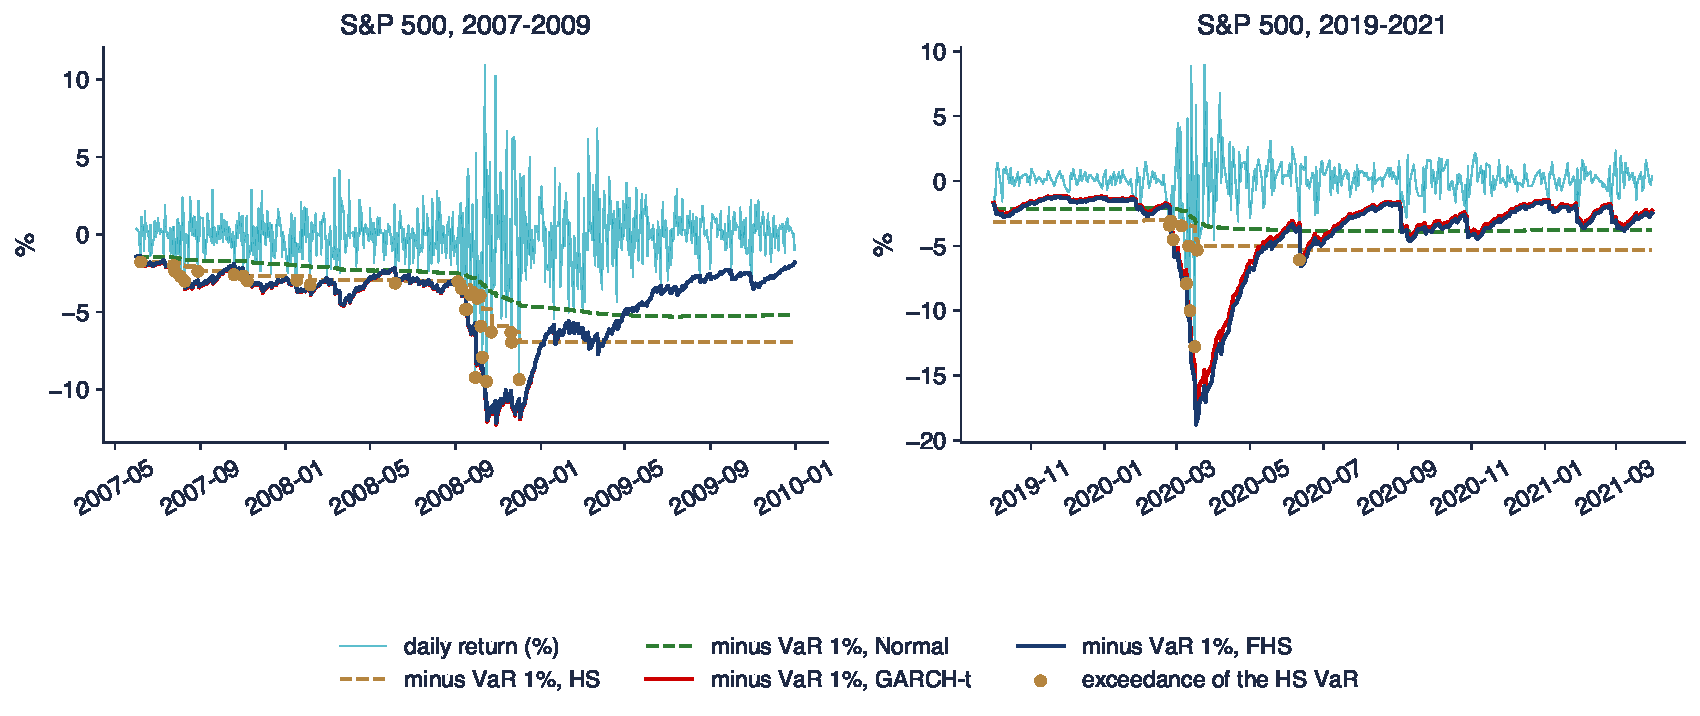
\includegraphics[width=0.97\textwidth,height=0.52\textheight,keepaspectratio]{sfm_ch10_rolling_var.pdf}
\end{center}
\vspace{-0.25cm}
\begin{itemize}
    \item S\&P 500: randamentele zilnice și minus prognozele VaR 1\% ale celor patru metode; punctele: depășirile VaR HS
    \item HS și metoda Normală reacționează cu luni de întîrziere: fereastra de 500 de zile se schimbă încet; GARCH-t și FHS cresc brusc în cîteva zile
    \item Interpretare: după criză, HS rămîne ridicat timp de doi ani (efectul de fantomă), în timp ce GARCH-t revine la niveluri normale
\end{itemize}
\sfmquantlet{Ch_10}{SFM_ch10_conditional_var}
\end{frame}

\begin{frame}{Perioade de stres: depășiri în 2008 și 2020}
\itemsize{\footnotesize}
\begin{center}
\footnotesize
\begin{tabular}{l|rrrr|r|rrrr|r}
\toprule
& \multicolumn{5}{c|}{sep. 2008 -- mar. 2009} & \multicolumn{5}{c}{feb. -- mai 2020} \\ & HS & Normală & GARCH-t & FHS & aștept. & HS & Normală & GARCH-t & FHS & aștept. \\
\midrule
S\&P 500 & 15 & 21 & 5 & 5 & 1{,}5 & 9 & 12 & 3 & 3 & 0{,}7 \\
DAX & 6 & 18 & 3 & 3 & 1{,}5 & 8 & 13 & 3 & 3 & 0{,}7 \\
BET & 8 & 14 & 4 & 4 & 1{,}4 & 5 & 10 & 4 & 4 & 0{,}7 \\
\bottomrule
\end{tabular}
\end{center}
\begin{itemize}
    \item Depășiri ale VaR 1\%: zile cu $r_t < -\mathrm{VaR}_t$; aștept.: 1\% din zilele perioadei
    \item În 2008, VaR Normal pentru S\&P 500 a fost depășit în 21 din 146 de zile, HS în 15; GARCH-t și FHS în 5
    \item Interpretare: nicio metodă nu este perfectă într-o criză, dar cele condiționate greșesc mult mai rar: prognoza volatilității contează mai mult decît forma cozii
\end{itemize}\sfmquantlet{Ch_10}{SFM_ch10_backtesting}
\end{frame}

\begin{frame}{Alegerea metodei}
\itemsize{\footnotesize}
\begin{center}
\footnotesize
\begin{tabular}{>{\raggedright\arraybackslash}p{3.6cm}>{\raggedright\arraybackslash}p{3.3cm}>{\raggedright\arraybackslash}p{4.0cm}}
\toprule
\textbf{Situația} & \textbf{Metoda} & \textbf{Motivul} \\
\midrule
VaR zilnic pentru o poziție lichidă & GARCH-t, FHS & urmăresc volatilitatea; FHS păstrează coada empirică \\
istoric lung, verificare rapidă & HS & fără model, ușor de explicat \\
$\alpha$ foarte mic (0,1\%), teste de stres & EVT & extrapolează dincolo de cea mai proastă zi \\
portofoliu cu multe active & varianță--covarianță, copulă & dependența; copula t pentru prăbușirile simultane \\
asimetrie și boltire moderate & Cornish--Fisher & o corecție rapidă a distribuției Normale \\
\bottomrule
\end{tabular}
\end{center}
\begin{itemize}
    \item Niciodată doar distribuția Normală pentru date zilnice; raportăm întotdeauna metoda, fereastra și nivelul
    \item Indiferent de metodă: o testăm prin backtesting (secțiunea 7)
\end{itemize}
\end{frame}

\begin{frame}{Recapitulare: VaR condiționat}
\itemsize{\small}
\begin{itemize}
    \item $\mathrm{VaR}_{t+1} = -(\mu + \sigma_{t+1}q_\alpha(z))$: GARCH-t ($z$ parametric) sau FHS ($z$ empiric)
    \item VaR condiționat urmărește furtunile; VaR pe fereastră întîrzie și păstrează fantomele
    \item În 2008 și 2020, metodele condiționate au avut de cîteva ori mai puține depășiri
\end{itemize}
\end{frame}


%=============================================================================
\section{VaR de portofoliu și dependența}
%=============================================================================

\begin{frame}{Un portofoliu BET și S\&P 500}
\itemsize{\small}
\begin{itemize}
    \item Ponderile $w = (0{,}5;\ 0{,}5)$; randamente simple $R_t$ în \%, astfel încît $R_{p,t} = w_1R_{1,t} + w_2R_{2,t}$ exact
    \begin{itemize}
        \item prețurile se aliniază pe cele 6\,466 de zile comune de tranzacționare din 2000, apoi se calculează randamentele
        \item fiecare indice în moneda lui: riscul valutar al unui investitor în lei este ignorat
    \end{itemize}
    \item Date zilnice: BET $\hat\mu = 0{,}076$, $\hat\sigma = 1{,}42$; S\&P 500 $\hat\mu = 0{,}034$, $\hat\sigma = 1{,}23$; corelația $\hat\rho = 0{,}21$
    \begin{itemize}
        \item BVB se închide înainte de deschiderea bursei din New York: o parte din reacția comună apare a doua zi, deci corelația din aceeași zi subestimează legătura
    \end{itemize}
    \item Întrebarea: este VaR-ul portofoliului mai mic decît media celor două VaR și cu cît?
\end{itemize}
\end{frame}

\begin{frame}{Metoda varianță--covarianță}
\itemsize{\footnotesize}
\begin{itemize}
    \item Portofoliul: $\mu_p = w^\top\mu$, $\sigma_p^2 = w^\top\Sigma w = w_1^2\sigma_1^2 + w_2^2\sigma_2^2 + 2w_1w_2\rho\sigma_1\sigma_2$ ($\Sigma$: matricea de covarianță)
    \begin{itemize}
        \item dacă randamentele sînt Normale în ansamblu: $\mathrm{VaR}_p = -(\mu_p + z_\alpha\sigma_p)$ (metoda RiskMetrics \refRM)
    \end{itemize}
    \item \textbf{Pas cu pas}: $\sigma_p^2 = 0{,}712^2 + 0{,}614^2 + 2 \times 0{,}5 \times 0{,}5 \times 0{,}369 = 1{,}068$, $\sigma_p = 1{,}033$
    \begin{itemize}
        \item VaR 1\% $= -(0{,}055 - 2{,}326 \times 1{,}033) = 2{,}35\%$; suma ponderată a celor două VaR Normale: $0{,}5 \times 3{,}23 + 0{,}5 \times 2{,}82 = 3{,}03\%$
        \item \textbf{beneficiul diversificării}: 22\% din risc dispare; cu $\rho = 1$ ar fi zero
    \end{itemize}
    \item Contribuțiile Euler $w_i(\Sigma w)_i/\sigma_p$ au suma $\sigma_p$: BET 56\%, S\&P 500 44\% din riscul portofoliului
\end{itemize}
\end{frame}

\begin{frame}{Corelația crește în crize}
\itemsize{\footnotesize}
\begin{center}
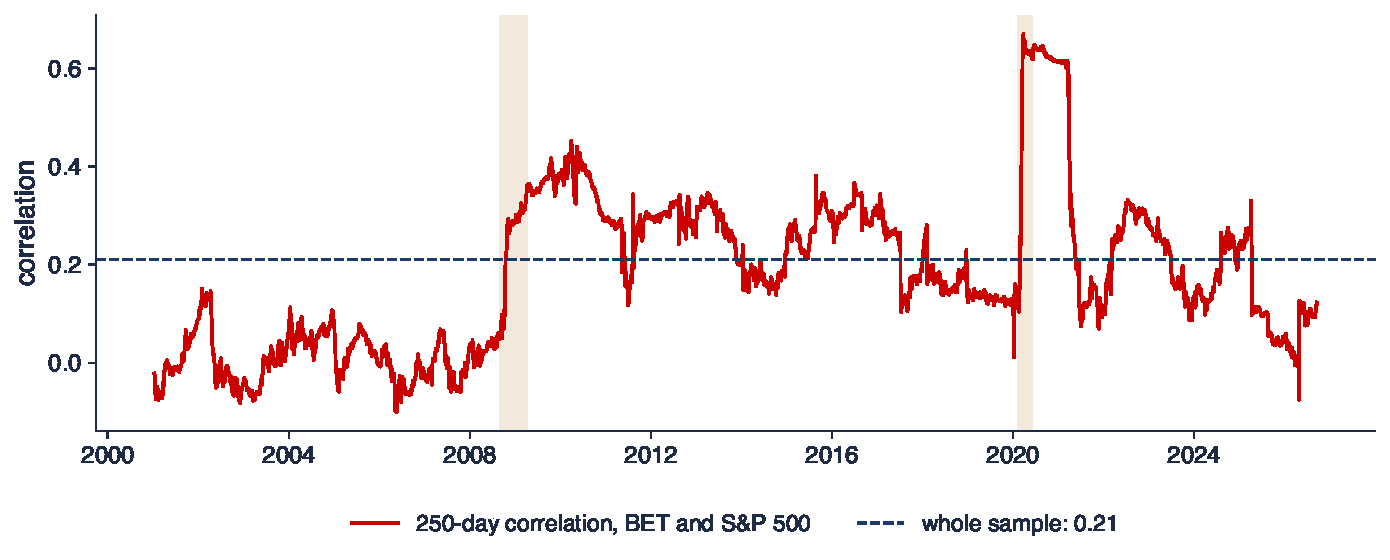
\includegraphics[width=0.97\textwidth,height=0.48\textheight,keepaspectratio]{sfm_ch10_rolling_corr.pdf}
\end{center}
\vspace{-0.25cm}
\begin{itemize}
    \item Corelația pe 250 de zile a randamentelor zilnice BET și S\&P 500; hașurat: perioadele de stres 2008 și 2020
    \item Anul liniștit 2017: $0{,}20$; septembrie 2008 -- martie 2009: $0{,}37$; februarie -- mai 2020: $0{,}71$; maximul $0{,}67$ la 25 martie 2020
    \item Interpretare: diversificarea este cea mai slabă exact cînd este nevoie de ea: un VaR construit pe corelația medie este prea optimist într-o criză
\end{itemize}
\sfmquantlet{Ch_10}{SFM_ch10_portfolio_copula}
\end{frame}

\begin{frame}{Corelația nu este dependență în cozi}
\itemsize{\small}
\begin{itemize}
    \item Corelația Pearson măsoară co-mișcarea liniară pe toate zilele; este dominată de zilele obișnuite \refEMS
    \begin{itemize}
        \item corelațiile de rang (Spearman, $\tau$ al lui Kendall) folosesc doar ordinea randamentelor: Kendall $\hat\tau = 0{,}100$, Spearman $0{,}15$
    \end{itemize}
    \item \textbf{Dependența în coada inferioară}: $\lambda_L = \lim_{q \to 0} P(U_1 \le q \mid U_2 \le q)$, $U_i = F_i(X_i)$ (randamentele pe o scală uniformă)
    \begin{itemize}
        \item șansa ca BET să aibă una dintre cele mai proaste zile ale lui, dat fiind că S\&P 500 are una dintre cele mai proaste zile ale lui
        \item datele: $q = 5\%$: $0{,}22$; $q = 1\%$: $0{,}19$; la independență, ambele ar fi egale cu $q$
    \end{itemize}
    \item Prăbușire simultană (ambele sub propria cuantilă de 1\%): 0{,}19\% dintre zile, față de 0{,}01\% la independență
\end{itemize}
\end{frame}

\begin{frame}{Copule: o introducere}
\itemsize{\small}
\begin{itemize}
    \item \textbf{Teorema lui Sklar}: orice funcție de repartiție comună se poate scrie $F(x_1, x_2) = C(F_1(x_1), F_2(x_2))$ \refQRM
    \begin{itemize}
        \item $F_1$, $F_2$: distribuțiile marginale (fiecare activ separat); $C$: \textbf{copula}, o distribuție comună a unor variabile uniforme pe $[0,1]^2$
        \item copula conține toată dependența, iar marginalele toate cozile individuale
    \end{itemize}
    \item Rețeta practică
    \begin{itemize}
        \item marginalele: empirice sau estimate (Student-t, EVT); dependența: o copulă estimată pe \textbf{pseudo-observațiile} $\hat U_{i,t} = \mathrm{rang}(X_{i,t})/(n + 1)$
        \item simulăm $(U_1, U_2)$ din copulă, revenim la randamente cu $F_i^{-1}$, calculăm randamentul portofoliului și citim VaR și ES
    \end{itemize}
    \item Manual: \refFHH, cap.~17
\end{itemize}
\end{frame}

\begin{frame}{Copula Gaussiană și copula t}
\itemsize{\footnotesize}
\begin{itemize}
    \item \textbf{Copula Gaussiană}: dependența unei distribuții Normale bivariate cu corelația $\rho$; $\lambda_L = 0$ pentru $\rho < 1$
    \begin{itemize}
        \item zilele extreme devin independente la limită: prăbușirile simultane sînt rare
    \end{itemize}
    \item \textbf{Copula t}: dependența unei distribuții Student-t bivariate cu $\rho$ și $\nu$ \refDM
    \begin{itemize}
        \item $\lambda_L = 2\,t_{\nu+1}\Big(-\sqrt{(\nu + 1)(1 - \rho)/(1 + \rho)}\Big) > 0$: prăbușirile apar împreună pe mai multe active
    \end{itemize}
    \item Estimarea pe BET și S\&P 500: $\rho = \sin(\pi\hat\tau/2) = 0{,}157$ (valabil pentru ambele copule); $\hat\nu = 4{,}50$ prin verosimilitate maximă
    \begin{itemize}
        \item log-verosimilitatea: Gaussiană $92{,}1$, t $219{,}5$; LR $= 254{,}9$, mult peste $\chi^2_{0{,}95}(1) = 3{,}84$: copula t este mai bună
        \item dependența în coadă implicată $\lambda_L = 0{,}096$, față de 0 pentru copula Gaussiană
    \end{itemize}
\end{itemize}
\end{frame}

\begin{frame}{Zile proaste comune: datele și două copule}
\itemsize{\footnotesize}
\begin{center}
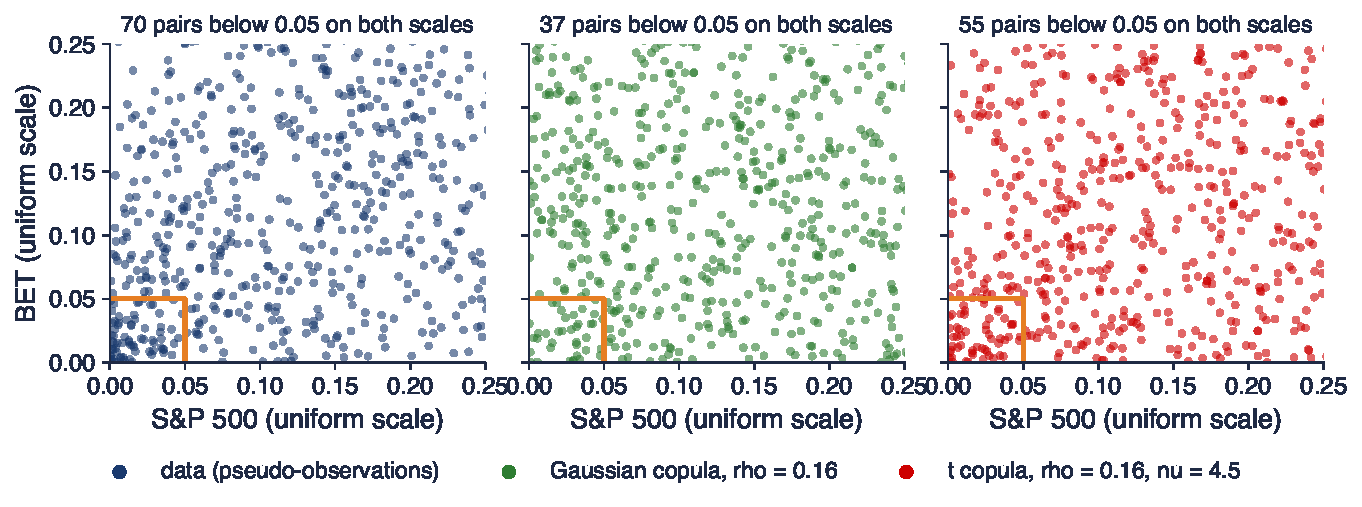
\includegraphics[width=0.97\textwidth,height=0.48\textheight,keepaspectratio]{sfm_ch10_copula.pdf}
\end{center}
\vspace{-0.25cm}
\begin{itemize}
    \item Colțul din stînga jos al scalei uniforme: pseudo-observațiile și eșantioane de aceeași mărime (6\,466) din copulele estimate
    \item Zile în care ambii indici sînt printre cele mai proaste 5\% ale lor: datele 70, Gaussiana 37, t 55; independența: circa 16
    \item Interpretare: copula Gaussiană înjumătățește numărul zilelor proaste comune; copula t este mult mai aproape de date
\end{itemize}
\sfmquantlet{Ch_10}{SFM_ch10_portfolio_copula}
\end{frame}

\begin{frame}{VaR prin copule: simularea pas cu pas}
\itemsize{\small}
\begin{itemize}
    \item \textbf{1.} Extragem $(Z_1, Z_2)$ dintr-o distribuție Normală bivariată cu corelația $\rho$
    \begin{itemize}
        \item copula Gaussiană: $U_i = \Phi(Z_i)$
        \item copula t: extragem $W \sim \chi^2_\nu$ și luăm $U_i = t_\nu(Z_i\sqrt{\nu/W})$: factorul comun $\sqrt{\nu/W}$ face ca extremele să apară împreună
    \end{itemize}
    \item \textbf{2.} Revenim la randamente cu funcțiile cuantilă empirice: $R_i = \hat F_i^{-1}(U_i)$
    \item \textbf{3.} Randamentul portofoliului $R_p = 0{,}5R_1 + 0{,}5R_2$; repetăm de 200\,000 de ori
    \item \textbf{4.} VaR 1\% și ES 2,5\% prin simulare istorică pe valorile simulate ale lui $R_p$
    \item Aceleași marginale în ambele copule: orice diferență de VaR vine numai din dependență
\end{itemize}\sfmquantlet{Ch_10}{SFM_ch10_portfolio_copula}
\end{frame}

\begin{frame}{VaR 1\% și ES 2,5\% ale portofoliului, pe metode}
\itemsize{\footnotesize}
\begin{center}
\footnotesize
\begin{tabular}{lrrr}
\toprule
Metoda & VaR 1\% & ES 2,5\% & P(prăbușire simultană la 1\%) \\
\midrule
varianță--covarianță (Normală) & $2{,}35$ & $2{,}36$ & -- \\
copula Gaussiană, marginale empirice & $2{,}75$ & $2{,}93$ & 0{,}03\% \\
copula t, marginale empirice & $2{,}81$ & $3{,}03$ & 0{,}13\% \\
simulare istorică (datele) & $3{,}08$ & $3{,}30$ & 0{,}19\% \\
\bottomrule
\end{tabular}
\end{center}
\begin{itemize}
    \item În \%, portofoliul 50/50, 6\,466 de zile comune; copule: 200\,000 de zile simulate
    \item Metoda Normală ignoră atît marginalele cu cozi groase, cît și dependența în cozi; copulele corectează marginalele, iar copula t și prăbușirile simultane
    \item Interpretare: copula t subestimează în continuare VaR istoric: legătura BET--S\&P 500 este mai puternică în crize decît poate descrie o copulă constantă
\end{itemize}\sfmquantlet{Ch_10}{SFM_ch10_portfolio_copula}
\end{frame}

\begin{frame}{Recapitulare: VaR de portofoliu și dependența}
\itemsize{\small}
\begin{itemize}
    \item Varianță--covarianță: $\sigma_p^2 = w^\top\Sigma w$; diversificarea reduce VaR cînd $\rho < 1$
    \item Corelația crește în crize; pentru prăbușirile simultane contează dependența în cozi
    \item Copula = dependența pe scala uniformă; copula t are dependență în cozi, cea Gaussiană nu are
\end{itemize}
\end{frame}


%=============================================================================
\section{Backtesting}
%=============================================================================

\begin{frame}{Ideea: secvența depășirilor}
\itemsize{\small}
\begin{itemize}
    \item \textbf{Depășire} (excepție): o zi cu $r_t < -\mathrm{VaR}_t$; $I_t = \mathbf{1}\{r_t < -\mathrm{VaR}_t\}$
    \begin{itemize}
        \item VaR trebuie să fie prognoza făcută cu o zi înainte: fără informații din viitor
    \end{itemize}
    \item Un VaR corect la nivelul $\alpha$: $I_t$ sînt i.i.d.\ Bernoulli($\alpha$) \refChris
    \begin{itemize}
        \item \textbf{acoperire necondiționată}: $P(I_t = 1) = \alpha$: numărul corect de depășiri
        \item \textbf{independență}: o depășire azi nu face mai probabilă o depășire mîine
    \end{itemize}
    \item Numărul de depășiri în $n$ zile: $x = \sum_t I_t \sim \mathrm{Binomial}(n, \alpha)$, media $n\alpha$, varianța $n\alpha(1 - \alpha)$
\end{itemize}
\end{frame}

\begin{frame}{Depășiri în 250 de zile pentru un VaR 1\% corect}
\itemsize{\footnotesize}
\begin{center}
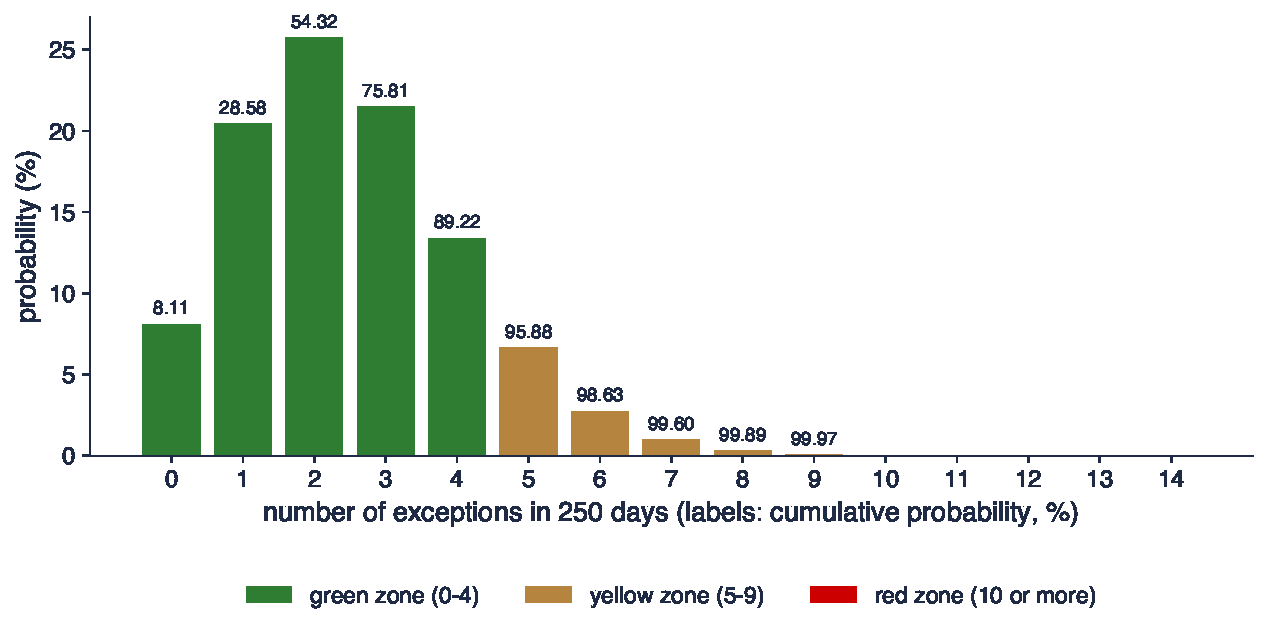
\includegraphics[width=0.97\textwidth,height=0.48\textheight,keepaspectratio]{sfm_ch10_binomial.pdf}
\end{center}
\vspace{-0.25cm}
\begin{itemize}
    \item $\mathrm{Binomial}(250; 0{,}01)$: 2,5 depășiri așteptate; 0 depășiri cu probabilitatea 8{,}11\%, 5 sau mai multe cu probabilitatea $100 - 89{,}22$, adică circa 11\%
    \item Interpretare: un an de date separă doar aproximativ un model bun de unul prost: un model corect ajunge în zona galbenă cam un an din nouă
\end{itemize}
\sfmquantlet{Ch_10}{SFM_ch10_backtesting}
\end{frame}

\begin{frame}{Testul POF al lui Kupiec}
\itemsize{\footnotesize}
\begin{itemize}
    \item \textbf{POF} (proportion of failures, proporția depășirilor) \refKupiec: $H_0$: $P(I_t = 1) = \alpha$; $\hat\pi = x/n$
    \begin{itemize}
        \item $LR_{uc} = -2\big[(n - x)\ln(1 - \alpha) + x\ln\alpha - (n - x)\ln(1 - \hat\pi) - x\ln\hat\pi\big] \sim \chi^2(1)$ sub $H_0$
        \item un test al raportului de verosimilitate (\sfmchlink{https://danpele.github.io/SFM/RO/Cursuri/capitol6_selectia_modelului_managementul_riscului.pdf}{Capitolul 6}); respingem la 5\% dacă $LR_{uc} > 3{,}84$
    \end{itemize}
    \item \textbf{Pas cu pas}: $n = 250$, $x = 7$, $\hat\pi = 0{,}028$
    \begin{itemize}
        \item $\ln L_0 = 243\ln 0{,}99 + 7\ln 0{,}01 = -34{,}68$; $\ln L_1 = 243\ln 0{,}972 + 7\ln 0{,}028 = -31{,}93$
        \item $LR_{uc} = -2(-34{,}68 - (-31{,}93)) = 5{,}50$, p $= 0{,}019$: respins la 5\%
    \end{itemize}
    \item Putere mică cu un an de date
    \begin{itemize}
        \item în 250 de zile, orice număr între 1 și 6 este acceptat la 5\%: un model cu o rată reală de 2\% trece testul cu probabilitatea 76\%
        \item și prea puține depășiri duc la respingere: un VaR exagerat de prudent irosește capital
    \end{itemize}
\end{itemize}
\end{frame}

\begin{frame}{Testul Kupiec pe 21 de ani de prognoze pentru S\&P 500}
\itemsize{\footnotesize}
\begin{itemize}
    \item VaR 1\% GARCH-t, 3 ianuarie 2005 -- 18 septembrie 2026: $n = 5\,460$ zile, $x = 95$ depășiri, $\hat\pi = 0{,}0174$
    \begin{itemize}
        \item așteptat $n\alpha = 55$; un interval binomial de 95\% pentru rată sub $H_0$: 0{,}75--1{,}26\%
    \end{itemize}
    \item \textbf{Pas cu pas}
    \begin{itemize}
        \item $\ln L_0 = 5365\ln 0{,}99 + 95\ln 0{,}01 = -491{,}4$
        \item $\ln L_1 = 5365\ln(1 - 0{,}0174) + 95\ln 0{,}0174 = -479{,}0$
        \item $LR_{uc} = -2(\ln L_0 - \ln L_1) = 24{,}73$, p $<$\,0{,}001
    \end{itemize}
    \item Interpretare: cu 21 de ani de date, chiar și o rată de 1{,}74\% în loc de 1\% este respinsă clar; o cauză probabilă este lipsa efectului de levier (\sfmchlink{https://danpele.github.io/SFM/RO/Cursuri/capitol9_modele_arch_garch.pdf}{Capitolul 9})
\end{itemize}\sfmquantlet{Ch_10}{SFM_ch10_backtesting}
\end{frame}

\begin{frame}{Testul de independență al lui Christoffersen}
\itemsize{\footnotesize}
\begin{itemize}
    \item Numărăm tranzițiile: $n_{ij}$ = numărul zilelor cu $I_{t-1} = i$ și $I_t = j$; $\hat\pi_{01} = \dfrac{n_{01}}{n_{00} + n_{01}}$, $\hat\pi_{11} = \dfrac{n_{11}}{n_{10} + n_{11}}$
    \begin{itemize}
        \item $H_0$: $\pi_{01} = \pi_{11}$ (o depășire azi nu schimbă șansa unei depășiri mîine) \refChris
        \item $LR_{ind} = -2\ln\dfrac{(1 - \hat\pi)^{n_{00} + n_{10}}\hat\pi^{n_{01} + n_{11}}}{(1 - \hat\pi_{01})^{n_{00}}\hat\pi_{01}^{n_{01}}(1 - \hat\pi_{11})^{n_{10}}\hat\pi_{11}^{n_{11}}} \sim \chi^2(1)$
    \end{itemize}
    \item \textbf{Acoperire condiționată}: $LR_{cc} = LR_{uc} + LR_{ind} \sim \chi^2(2)$; respingem la 5\% dacă $LR_{cc} > 5{,}99$
    \item \textbf{Exemplu}: S\&P 500, VaR 1\% HS, 5\,460 de zile: $n_{00} = 5313$, $n_{01} = 69$, $n_{10} = 69$, $n_{11} = 8$
    \begin{itemize}
        \item $\hat\pi_{01} = 1{,}28\%$, $\hat\pi_{11} = 10{,}4\%$: după o depășire, următoarea este de 8 ori mai probabilă
        \item $LR_{ind} = 19{,}43$ (p $<$\,0{,}001): depășirile apar grupat
    \end{itemize}
\end{itemize}
\end{frame}

\begin{frame}{Semaforul Basel}
\itemsize{\footnotesize}
\begin{columns}[T]
\begin{column}{0.44\textwidth}
\begin{center}
\scriptsize
\begin{tabular}{lcrrr}
\toprule
$x$ & Zona & Cumul.\ (\%) & Adaos & Factor \\
\midrule
0 & verde & $8{,}11$ & $0{,}00$ & $3{,}00$ \\
1 & verde & $28{,}58$ & $0{,}00$ & $3{,}00$ \\
2 & verde & $54{,}32$ & $0{,}00$ & $3{,}00$ \\
3 & verde & $75{,}81$ & $0{,}00$ & $3{,}00$ \\
4 & verde & $89{,}22$ & $0{,}00$ & $3{,}00$ \\
5 & galbenă & $95{,}88$ & $0{,}40$ & $3{,}40$ \\
6 & galbenă & $98{,}63$ & $0{,}50$ & $3{,}50$ \\
7 & galbenă & $99{,}60$ & $0{,}65$ & $3{,}65$ \\
8 & galbenă & $99{,}89$ & $0{,}75$ & $3{,}75$ \\
9 & galbenă & $99{,}97$ & $0{,}85$ & $3{,}85$ \\
$\ge 10$ & roșie & $99{,}99$ & $1{,}00$ & $4{,}00$ \\
\bottomrule
\end{tabular}
\end{center}

\end{column}
\begin{column}{0.54\textwidth}
\begin{itemize}
    \item \refBCBSb: se numără depășirile VaR 1\% pe o zi în ultimele 250 de zile
    \begin{itemize}
        \item verde: nicio măsură; galbenă: factorul crește cu adaosul; roșie: modelul este considerat greșit
    \end{itemize}
    \item Capitalul $= (3 + \text{adaos}) \times$ media pe 60 de zile a VaR 1\% pe 10 zile (sau valoarea de ieri, dacă este mai mare)
    \begin{itemize}
        \item zonele vin din distribuția binomială: zona galbenă începe unde probabilitatea cumulată trece de 95\%, zona roșie unde atinge 99,99\%
    \end{itemize}
    \item $x$: depășiri în 250 de zile; Cumul.: $P(X \le x)$ pentru $\mathrm{Binomial}(250; 0{,}01)$
    \item FRTB păstrează numărarea depășirilor VaR 1\% la nivelul băncii și al diviziilor \refMARb
\end{itemize}
\end{column}
\end{columns}
\end{frame}

\begin{frame}{Depășirile în timp}
\itemsize{\footnotesize}
\begin{center}
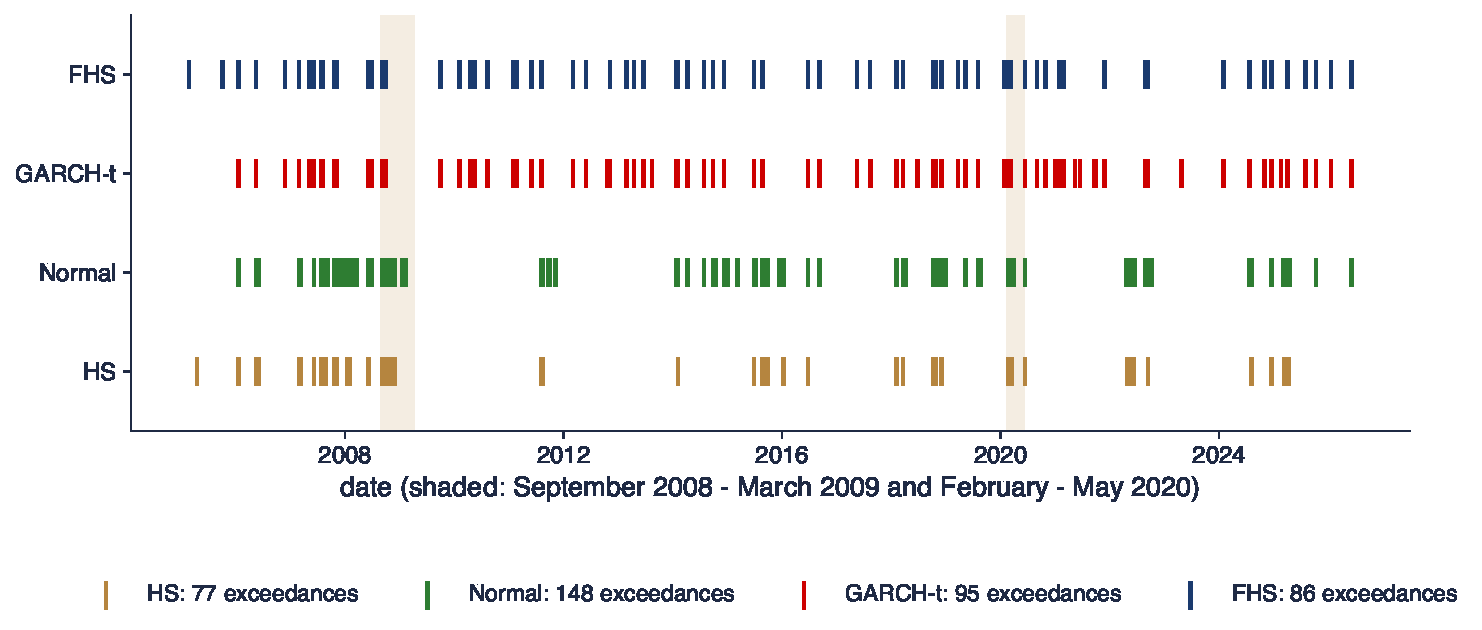
\includegraphics[width=0.97\textwidth,height=0.48\textheight,keepaspectratio]{sfm_ch10_hits.pdf}
\end{center}
\vspace{-0.25cm}
\begin{itemize}
    \item S\&P 500, 2005--2026: fiecare marcaj este o zi în care VaR 1\% al metodei a fost depășit; aproximativ 55 așteptate pentru fiecare metodă
    \item Interpretare: depășirile HS și Normale vin în rafale (2007--2008, 2011, 2022); depășirile GARCH-t și FHS sînt răspîndite în timp, dar sînt mai multe în anii liniștiți
\end{itemize}
\sfmquantlet{Ch_10}{SFM_ch10_backtesting}
\end{frame}

\begin{frame}{Rezultatele backtesting-ului: S\&P 500 și DAX}
\itemsize{\footnotesize}
\begin{center}
\scriptsize
\begin{tabular}{llrrrrrrr}
\toprule
& Metoda & $x$ & rata (\%) & p POF & p ind. & p ac.c. & max. 250 z. & $Z_2$ (p) \\
\midrule
S\&P 500 & HS & 77 & $1{,}41$ & 0{,}004 & $<$\,0{,}001 & $<$\,0{,}001 & 18 & ${-0{,}39}$ ($<$\,0{,}001) \\
 & Normal & 148 & $2{,}71$ & $<$\,0{,}001 & $<$\,0{,}001 & $<$\,0{,}001 & 29 & ${-1{,}15}$ ($<$\,0{,}001) \\
 & GARCH-t & 95 & $1{,}74$ & $<$\,0{,}001 & 0{,}114 & $<$\,0{,}001 & 10 & ${-0{,}54}$ ($<$\,0{,}001) \\
 & FHS & 86 & $1{,}58$ & $<$\,0{,}001 & 0{,}060 & $<$\,0{,}001 & 10 & ${-0{,}20}$ (0{,}013) \\
\midrule
DAX & HS & 67 & $1{,}21$ & 0{,}121 & $<$\,0{,}001 & $<$\,0{,}001 & 12 & ${-0{,}26}$ (0{,}002) \\
 & Normal & 133 & $2{,}41$ & $<$\,0{,}001 & $<$\,0{,}001 & $<$\,0{,}001 & 19 & ${-0{,}87}$ ($<$\,0{,}001) \\
 & GARCH-t & 84 & $1{,}52$ & $<$\,0{,}001 & 0{,}549 & 0{,}001 & 9 & ${-0{,}49}$ ($<$\,0{,}001) \\
 & FHS & 77 & $1{,}40$ & 0{,}005 & 0{,}418 & 0{,}015 & 9 & ${-0{,}18}$ (0{,}014) \\
\bottomrule
\end{tabular}
\end{center}
\begin{itemize}
    \item VaR 1\% din 3 ianuarie 2005 (circa 5\,500 de zile); $x$: depășirile; p ind.: independența Christoffersen; p ac.c.: acoperirea condiționată; max. 250 z.: cel mai mare număr pe 250 de zile
    \item Distribuția Normală: respinsă peste tot; HS: depășirile apar grupat; GARCH-t și FHS: depășiri independente, dar o rată de 1{,}4--1{,}7\%
\end{itemize}\sfmquantlet{Ch_10}{SFM_ch10_backtesting}
\end{frame}

\begin{frame}{Rezultatele backtesting-ului: BET și Bitcoin}
\itemsize{\footnotesize}
\begin{center}
\scriptsize
\begin{tabular}{llrrrrrrr}
\toprule
& Metoda & $x$ & rata (\%) & p POF & p ind. & p ac.c. & max. 250 z. & $Z_2$ (p) \\
\midrule
BET & HS & 66 & $1{,}22$ & 0{,}123 & 0{,}001 & 0{,}002 & 14 & ${-0{,}27}$ (0{,}001) \\
 & Normal & 122 & $2{,}25$ & $<$\,0{,}001 & $<$\,0{,}001 & $<$\,0{,}001 & 21 & ${-0{,}83}$ ($<$\,0{,}001) \\
 & GARCH-t & 65 & $1{,}20$ & 0{,}158 & 0{,}807 & 0{,}358 & 9 & ${-0{,}22}$ (0{,}007) \\
 & FHS & 65 & $1{,}20$ & 0{,}158 & 0{,}240 & 0{,}185 & 7 & ${-0{,}18}$ (0{,}021) \\
\midrule
Bitcoin & HS & 33 & $0{,}93$ & 0{,}672 & 0{,}316 & 0{,}553 & 6 & ${-0{,}07}$ (0{,}224) \\
 & Normal & 69 & $1{,}94$ & $<$\,0{,}001 & 0{,}057 & $<$\,0{,}001 & 16 & ${-0{,}56}$ ($<$\,0{,}001) \\
 & GARCH-t & 48 & $1{,}35$ & 0{,}045 & 0{,}683 & 0{,}123 & 8 & ${-0{,}41}$ ($<$\,0{,}001) \\
 & FHS & 24 & $0{,}68$ & 0{,}040 & 0{,}155 & 0{,}044 & 6 & ${0{,}12}$ (0{,}834) \\
\bottomrule
\end{tabular}
\end{center}
\begin{itemize}
    \item VaR 1\% din 3 ianuarie 2005 (Bitcoin din 1 ianuarie 2017); $x$: depășirile; p ind.: independența Christoffersen; p ac.c.: acoperirea condiționată; max. 250 z.: cel mai mare număr pe 250 de zile
    \item BET: GARCH-t și FHS trec toate cele trei teste; Bitcoin: HS trece testele, FHS este prea prudent ($0{,}68\%$)
\end{itemize}\sfmquantlet{Ch_10}{SFM_ch10_backtesting}
\end{frame}

\begin{frame}{Ordonarea prognozelor și zona de azi}
\itemsize{\footnotesize}
\begin{center}
\footnotesize
\begin{tabular}{l|rrrr|rrrr}
\toprule
& \multicolumn{4}{c|}{pierderea cuantilă medie $\times 100$} & \multicolumn{4}{c}{depășiri, ultimele 250 de zile} \\ & HS & Normală & GARCH-t & FHS & HS & Normală & GARCH-t & FHS \\
\midrule
S\&P 500 & $5{,}17$ & $5{,}80$ & $3{,}71$ & $3{,}68$ & 0 & 2 & 3 & 3 \\
DAX & $5{,}15$ & $5{,}52$ & $4{,}08$ & $4{,}05$ & 1 & 3 & 3 & 3 \\
BET & $6{,}04$ & $6{,}26$ & $4{,}59$ & $4{,}62$ & 4 & 6 & 3 & 2 \\
Bitcoin & $13{,}57$ & $14{,}52$ & $13{,}53$ & $13{,}75$ & 3 & 4 & 2 & 2 \\
\bottomrule
\end{tabular}
\end{center}
\begin{itemize}
    \item Testele spun dacă un model este acceptabil; o \textbf{funcție de scor} spune care dintre două modele este mai bun
    \begin{itemize}
        \item VaR este elicitabil: media pierderii cuantile $\frac1n\sum_t(\alpha - I_t)(r_t + \mathrm{VaR}_t)$ ordonează prognozele \refGneiting
    \end{itemize}
    \item Indicii de acțiuni: GARCH-t și FHS au pierderea cea mai mică, metoda Normală cea mai mare; Bitcoin: cele patru metode sînt apropiate
    \item Interpretare: în ultimele 250 de zile, toate modelele sînt în zona verde, cu excepția VaR Normal pentru BET (6, zona galbenă): o fereastră recentă spune puțin despre un model
\end{itemize}\sfmquantlet{Ch_10}{SFM_ch10_backtesting}
\end{frame}

\begin{frame}{Semaforul Basel în timp}
\itemsize{\footnotesize}
\begin{center}
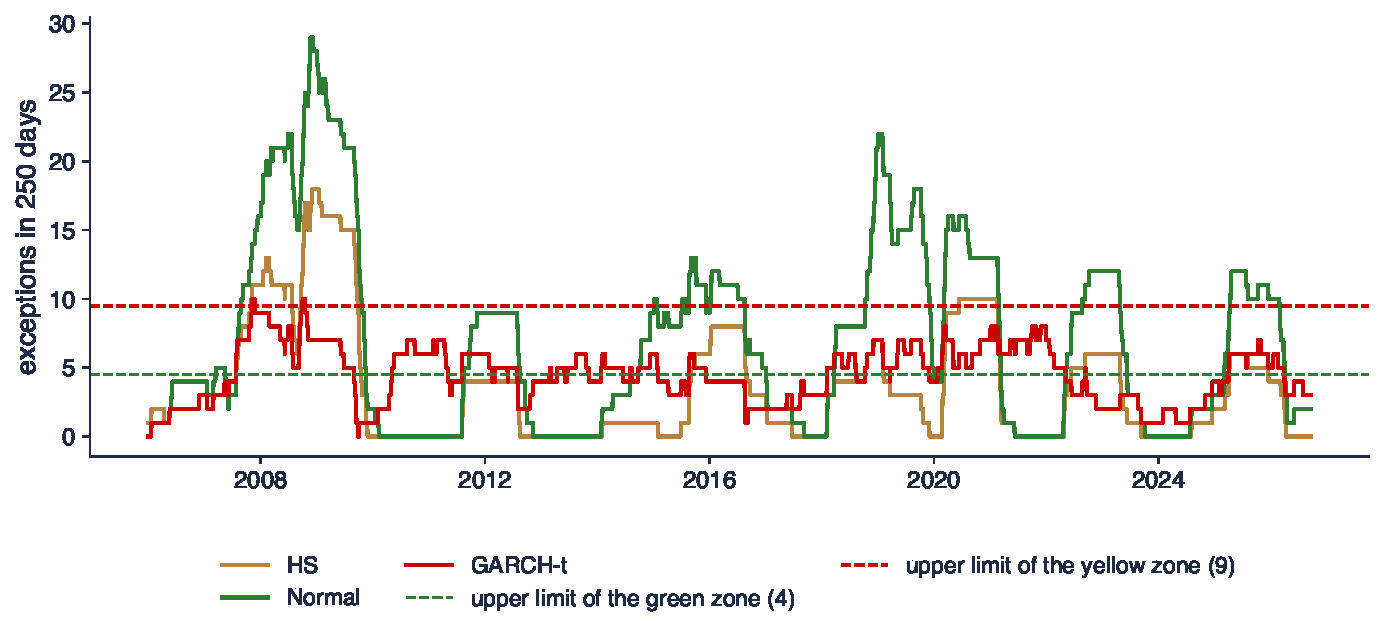
\includegraphics[width=0.97\textwidth,height=0.48\textheight,keepaspectratio]{sfm_ch10_traffic_time.pdf}
\end{center}
\vspace{-0.25cm}
\begin{itemize}
    \item S\&P 500: numărul depășirilor VaR 1\% în ultimele 250 de zile, pentru fiecare zi din 2006; linii întrerupte: limitele zonelor
    \item Ponderea zilelor în zona roșie: Normală 33\%, HS 12\%, GARCH-t 0\%; cel mai mare număr: 29, 18 și 10
    \item Interpretare: o bancă ce ar fi folosit VaR Normal sau HS ar fi plătit penalizarea zonei roșii în cea mai mare parte din 2008--2009; GARCH-t aproape că nu ajunge niciodată în zona roșie
\end{itemize}
\sfmquantlet{Ch_10}{SFM_ch10_backtesting}
\end{frame}

\begin{frame}{Backtesting pentru ES: Acerbi și Székely}
\itemsize{\footnotesize}
\begin{itemize}
    \item ES nu este elicitabil singur, dar poate fi testat împreună cu VaR \refAS
    \begin{itemize}
        \item $Z_2 = \dfrac{1}{T\alpha}\displaystyle\sum_{t=1}^{T}\dfrac{r_t I_t}{\mathrm{ES}_t} + 1$, \quad $I_t = \mathbf{1}\{r_t < -\mathrm{VaR}_t\}$, $\alpha = 2{,}5\%$
        \item dacă VaR și ES sînt corecte, $E[Z_2] = 0$; $Z_2 < 0$: pierderile de dincolo de VaR sînt mai mari decît ES prognozat sau prea dese
    \end{itemize}
    \item p-valoarea prin simulare: extragem randamente din distribuția prognozată a fiecărei zile și recalculăm $Z_2$ de 1000 de ori
    \begin{itemize}
        \item S\&P 500: Normală $Z_2 = -1{,}15$, HS $-0{,}39$, GARCH-t $-0{,}54$, FHS $-0{,}20$ (p 0{,}013)
    \end{itemize}
    \item Interpretare: toate cele patru prognoze ES 2,5\% sînt prea mici pentru indicii de acțiuni; FHS este cel mai aproape, deoarece preia coada lui $z$ din date
\end{itemize}\sfmquantlet{Ch_10}{SFM_ch10_backtesting}
\end{frame}

\begin{frame}{Studiu de caz: modelele VaR ale băncilor comerciale}
\itemsize{\small}
\begin{itemize}
    \item \refBO: primul studiu al prognozelor VaR raportate efectiv de mari bănci americane, comparate cu P\&L-ul zilnic din tranzacționare
    \begin{itemize}
        \item designul: VaR 1\% al băncilor față de P\&L-ul realizat; un model GARCH simplu al P\&L-ului fiecărei bănci ca reper
    \end{itemize}
    \item Rezultatele
    \begin{itemize}
        \item VaR-ul băncilor a fost în medie prudent, dar depășirile care au avut loc au apărut grupat
        \item reperul GARCH a dat valori VaR mai mici, cu o acoperire comparabilă: a urmărit mai bine schimbările volatilității
    \end{itemize}
    \item Același tipar ca în datele noastre: VaR-ul pe fereastră este fie prea mare în perioadele liniștite, fie prea lent în furtuni; VaR condiționat se adaptează
    \item Lectură suplimentară despre prognoza directă a cuantilei: CAViaR \refCAViaR
\end{itemize}
\end{frame}

\begin{frame}{Recapitulare: backtesting}
\itemsize{\small}
\begin{itemize}
    \item Depășirile trebuie să fie Bernoulli($\alpha$) și independente: Kupiec testează rata, Christoffersen gruparea
    \item Semaforul Basel: 0--4 verde, 5--9 galben, 10 sau mai multe roșu, în 250 de zile
    \item ES se testează împreună cu VaR ($Z_2$); metodele condiționate trec testele mai des decît cele pe fereastră
\end{itemize}
\end{frame}


%=============================================================================
\section{AI pentru descoperire științifică}
%=============================================================================

\begin{frame}{O întrebare deschisă}
\itemsize{\small}
\begin{itemize}
    \item \textbf{Crește brusc dependența în cozi dintre BVB și piețele mondiale în crize și revine apoi la nivelul anterior?}
    \begin{itemize}
        \item azi: corelația $0{,}20$ într-un an liniștit, $0{,}71$ în primăvara lui 2020; o copulă t constantă dă $\lambda_L = 0{,}096$
        \item un VaR de portofoliu cu o copulă constantă rămîne sub cel istoric (secțiunea precedentă)
    \end{itemize}
    \item Întrebarea rămîne deschisă: crizele sînt puține, BVB se tranzacționează la alte ore, iar estimările din coadă au nevoie de multe observații
    \item Lucrări înrudite despre entropie ca măsură de risc, ca lectură suplimentară: \refPeleA; \refPeleB
    \item Instrumentele AI pot accelera un astfel de studiu; nu înlocuiesc verificarea lui \refWang
\end{itemize}
\end{frame}

\begin{frame}{Contribuția posibilă a AI}
\itemsize{\small}
\begin{itemize}
    \item \textbf{Literatura}: o listă a studiilor despre copule variabile în timp și despre contagiunea dintre piețele emergente și cele dezvoltate
    \item \textbf{Cod}: o primă versiune a estimărilor copulei t pe ferestre mobile (250 de zile) pentru BET și S\&P 500, cu $\rho$, $\nu$ și $\lambda_L$ în timp
    \item \textbf{Robustețe}: randamente pe două zile (ore de tranzacționare diferite), DAX în loc de S\&P 500, alte ferestre
    \item Exemplu de prompt
    \begin{itemize}
        \item \aiprompt{Write Python code that fits a bivariate t copula by maximum likelihood to the pseudo-observations of daily BET and S\&P 500 returns on rolling windows of 250 days moved by 21 days, and plots rho, nu and the lower tail dependence over time.}
    \end{itemize}
\end{itemize}
\end{frame}

\begin{frame}{Verificări necesare}
\itemsize{\small}
\begin{itemize}
    \item Convenția VaR: „VaR 1\%” este pierderea depășită cu probabilitatea 1\%, un număr pozitiv; un răspuns care folosește probabilitatea complementară sau raportează un VaR negativ amestecă convențiile
    \item Prețurile se aliniază pe zilele comune înainte de calculul randamentelor; BVB și New York se tranzacționează la ore diferite
    \item Pseudo-observațiile: rangurile împărțite la $n + 1$, nu la $n$ (altfel densitatea copulei este infinită în 1)
    \item Dependența în cozi din 250 de zile se bazează pe cîteva zile proaste comune: raportați incertitudinea ei (bootstrap, \sfmchlink{https://danpele.github.io/SFM/RO/Cursuri/capitol2_distributii_clasice_fapte_stilizate.pdf}{Capitolul 2})
    \item Ferestrele suprapuse: estimările consecutive nu sînt dovezi independente
    \item Referințele: fiecare lucrare citată trebuie să existe; verificați DOI-ul
\end{itemize}
\end{frame}

\begin{frame}{Idee de proiect}
\itemsize{\small}
\begin{itemize}
    \item \textbf{Întrebarea}: dă o copulă variabilă în timp un VaR de portofoliu mai bun decît o copulă constantă, pentru un portofoliu BVB și acțiuni mondiale?
    \begin{itemize}
        \item date: BET, BET-TR, S\&P 500, DAX din 2005 (EODHD)
    \end{itemize}
    \item Pași
    \begin{itemize}
        \item marginale GARCH-t pentru fiecare indice (\sfmchlink{https://danpele.github.io/SFM/RO/Cursuri/capitol9_modele_arch_garch.pdf}{Capitolul 9}); copulă t constantă și pe fereastră mobilă pentru dependență
        \item VaR 1\% și ES 2,5\% pe o zi pentru un portofoliu 50/50, în afara eșantionului, din 2008
        \item testele Kupiec, Christoffersen și $Z_2$ pentru ambele variante, cu atenție specială pentru 2008, 2020 și 2022
    \end{itemize}
    \item Livrabil: un tabel, un grafic și un paragraf despre ce pot și ce nu pot arăta datele
    \item Declarați orice utilizare a instrumentelor AI și enumerați erorile acestora pe care le-ați corectat
\end{itemize}
\end{frame}


%=============================================================================
\section{Rezumat}
%=============================================================================

\begin{frame}{Idei de reținut}
\itemsize{\small}
\begin{itemize}
    \item VaR 1\% $= -q_{1\%}$: pierderea depășită într-o zi din o sută; ES 2,5\%: pierderea medie din cele mai proaste 2,5\% dintre zile
    \item ES este coerent; VaR poate penaliza diversificarea; VaR este elicitabil, ES doar împreună cu VaR
    \item VaR-ul Normal este prea mic cu 14--24\% pe date zilnice; HS, Student-t și EVT sînt de acord la 1\%; Cornish--Fisher nu funcționează pentru boltire mare
    \item VaR condiționat (GARCH-t, FHS) urmărește furtunile și trece testele pe care metodele pe fereastră nu le trec
    \item Riscul de portofoliu: corelația crește în crize; dependența în cozi (copula t) contează pentru prăbușirile simultane
    \item Backtesting cu Kupiec (rata), Christoffersen (gruparea), semaforul Basel (reglementarea) și $Z_2$ (ES)
\end{itemize}
\end{frame}

\begin{frame}{Formule de reținut}
\itemsize{\small}
{\renewcommand{\arraystretch}{1.45}\begin{center}
\scriptsize
\begin{tabular}{ll}
\toprule
\textbf{Mărimea} & \textbf{Formula} \\
\midrule
VaR & $\mathrm{VaR}_\alpha = -q_\alpha(X)$; \ HS: $-r_{(\lceil n\alpha\rceil)}$ \\
ES & $\mathrm{ES}_\alpha = -\frac{1}{\alpha}\int_0^\alpha q_u\,du$; \ HS: $-\frac1k\sum_{i \le k} r_{(i)}$ \\
Normală & $-(\mu + \sigma z_\alpha)$, \ $-\mu + \sigma\varphi(z_\alpha)/\alpha$ \\
EVT (POT) & $u + \frac{\beta}{\xi}[(n\alpha/N_u)^{-\xi} - 1]$, \ ES $= (\mathrm{VaR} + \beta - \xi u)/(1 - \xi)$ \\
Condiționat & $-(\mu + \sigma_{t+1}q_\alpha(z))$ \\
Portofoliu & $\sigma_p^2 = w^\top\Sigma w$ \\
t copula & $\lambda_L = 2t_{\nu+1}(-\sqrt{(\nu + 1)(1 - \rho)/(1 + \rho)})$ \\
Kupiec & $LR_{uc} = -2\ln[(1-\alpha)^{n-x}\alpha^x/((1-\hat\pi)^{n-x}\hat\pi^x)] \sim \chi^2(1)$ \\
Christoffersen & $LR_{cc} = LR_{uc} + LR_{ind} \sim \chi^2(2)$ \\
Acerbi--Székely & $Z_2 = \frac{1}{T\alpha}\sum_t r_tI_t/\mathrm{ES}_t + 1$ \\
\bottomrule
\end{tabular}
\end{center}
}
\end{frame}

\begin{frame}{Autoevaluare}
\itemsize{\small}
\begin{itemize}
    \item \textbf{Întrebare}: o divizie raportează „VaR 1\% = $-2{,}4\%$”. Ce este greșit?
    \begin{itemize}
        \item \textbf{Răspuns}: semnul: $-2{,}4\%$ este cuantila $q_{0{,}01}$; VaR 1\% $= -q_{0{,}01} = 2{,}4\%$, o pierdere
    \end{itemize}
    \item \textbf{Întrebare}: un model are 3 depășiri în 250 de zile, toate în aceeași săptămînă. Ce test detectează problema?
    \begin{itemize}
        \item \textbf{Răspuns}: nu testul Kupiec (3 este aproape de 2,5), ci testul de independență al lui Christoffersen
    \end{itemize}
    \item \textbf{Întrebare}: două portofolii au același VaR 1\%. Pot avea ES 2,5\% diferit?
    \begin{itemize}
        \item \textbf{Răspuns}: da: ES depinde de întreaga coadă de dincolo de cuantilă, VaR doar de un punct
    \end{itemize}
    \item Urmează: Capitolul 11, ipoteza piețelor fractale și memoria lungă
\end{itemize}
\end{frame}


%=============================================================================
\section{Bibliografie}
%=============================================================================

\begin{frame}{Bibliografie (1/2)}
\itemsize{\tiny}
\begin{itemize}
    \item Acerbi, C., Székely, B. (2014). \href{https://www.msci.com/documents/10199/22aa9922-f874-4060-b77a-0f0e267a489b}{Backtesting expected shortfall}. MSCI Research; published in \textit{Risk}, December 2014.
    \item Acerbi, C., Tasche, D. (2002). \href{https://doi.org/10.1016/S0378-4266(02)00283-2}{On the coherence of expected shortfall}. \textit{Journal of Banking \& Finance}, 26(7), 1487--1503.
    \item Artzner, P., Delbaen, F., Eber, J.-M., Heath, D. (1999). \href{https://doi.org/10.1111/1467-9965.00068}{Coherent measures of risk}. \textit{Mathematical Finance}, 9(3), 203--228.
    \item Barone-Adesi, G., Giannopoulos, K., Vosper, L. (1999). \href{https://doi.org/10.1002/(SICI)1096-9934(199908)19:5<583::AID-FUT5>3.0.CO;2-S}{VaR without correlations for portfolios of derivative securities}. \textit{Journal of Futures Markets}, 19(5), 583--602.
    \item Basel Committee on Banking Supervision (1996a). \href{https://www.bis.org/publ/bcbs24.htm}{Amendment to the capital accord to incorporate market risks}. Bank for International Settlements.
    \item Basel Committee on Banking Supervision (1996b). \href{https://www.bis.org/publ/bcbs22.htm}{Supervisory framework for the use of ``backtesting'' in conjunction with the internal models approach to market risk capital requirements}. Bank for International Settlements.
    \item Basel Committee on Banking Supervision (2019). \href{https://www.bis.org/bcbs/publ/d457.htm}{Minimum capital requirements for market risk}. Bank for International Settlements.
    \item Berkowitz, J., O'Brien, J. (2002). \href{https://doi.org/10.1111/1540-6261.00455}{How accurate are value-at-risk models at commercial banks?} \textit{Journal of Finance}, 57(3), 1093--1111.
    \item Bollerslev, T. (1986). \href{https://doi.org/10.1016/0304-4076(86)90063-1}{Generalized autoregressive conditional heteroskedasticity}. \textit{Journal of Econometrics}, 31(3), 307--327.
    \item Borak, S., Härdle, W.K., López-Cabrera, B. (2013). \href{https://doi.org/10.1007/978-3-642-33929-5}{\textit{Statistics of Financial Markets: Exercises and Solutions}}, 2nd ed. Springer.
    \item Christoffersen, P.F. (1998). \href{https://doi.org/10.2307/2527341}{Evaluating interval forecasts}. \textit{International Economic Review}, 39(4), 841--862.
    \item Cornish, E.A., Fisher, R.A. (1938). \href{https://doi.org/10.2307/1400905}{Moments and cumulants in the specification of distributions}. \textit{Revue de l'Institut International de Statistique}, 5(4), 307--320.
    \item Daníelsson, J., Jorgensen, B.N., Samorodnitsky, G., Sarma, M., de Vries, C.G. (2013). \href{https://doi.org/10.1016/j.jeconom.2012.08.011}{Fat tails, VaR and subadditivity}. \textit{Journal of Econometrics}, 172(2), 283--291.
    \item Demarta, S., McNeil, A.J. (2005). \href{https://doi.org/10.1111/j.1751-5823.2005.tb00254.x}{The t copula and related copulas}. \textit{International Statistical Review}, 73(1), 111--129.
    \item Embrechts, P., McNeil, A.J., Straumann, D. (2002). \href{https://doi.org/10.1017/CBO9780511615337.008}{Correlation and dependence in risk management: properties and pitfalls}. In M. Dempster (ed.), \textit{Risk Management: Value at Risk and Beyond}, 176--223. Cambridge University Press.
    \item Engle, R.F., Manganelli, S. (2004). \href{https://doi.org/10.1198/073500104000000370}{CAViaR: conditional autoregressive value at risk by regression quantiles}. \textit{Journal of Business \& Economic Statistics}, 22(4), 367--381.
\end{itemize}
\end{frame}

\begin{frame}{Bibliografie (2/2)}
\itemsize{\tiny}
\begin{itemize}
    \item Fissler, T., Ziegel, J.F. (2016). \href{https://doi.org/10.1214/16-AOS1439}{Higher order elicitability and Osband's principle}. \textit{Annals of Statistics}, 44(4), 1680--1707.
    \item Franke, J., Härdle, W.K., Hafner, C.M. (2019). \href{https://doi.org/10.1007/978-3-030-13751-9}{\textit{Statistics of Financial Markets: An Introduction}}, 5th ed. Springer.
    \item Gneiting, T. (2011). \href{https://doi.org/10.1198/jasa.2011.r10138}{Making and evaluating point forecasts}. \textit{Journal of the American Statistical Association}, 106(494), 746--762.
    \item Hull, J., White, A. (1998). \href{https://doi.org/10.21314/JOR.1998.001}{Incorporating volatility updating into the historical simulation method for value-at-risk}. \textit{Journal of Risk}, 1(1), 5--19.
    \item J.P. Morgan/Reuters (1996). \href{https://www.msci.com/documents/10199/5915b101-4206-4ba0-aee2-3449d5c7e95a}{\textit{RiskMetrics -- Technical Document}}, 4th ed. New York.
    \item Kupiec, P.H. (1995). \href{https://doi.org/10.3905/jod.1995.407942}{Techniques for verifying the accuracy of risk measurement models}. \textit{Journal of Derivatives}, 3(2), 73--84.
    \item McNeil, A.J., Frey, R. (2000). \href{https://doi.org/10.1016/S0927-5398(00)00012-8}{Estimation of tail-related risk measures for heteroscedastic financial time series: an extreme value approach}. \textit{Journal of Empirical Finance}, 7(3--4), 271--300.
    \item McNeil, A.J., Frey, R., Embrechts, P. (2015). \href{https://press.princeton.edu/books/hardcover/9780691166278/quantitative-risk-management}{\textit{Quantitative Risk Management: Concepts, Techniques and Tools}}, revised ed. Princeton University Press.
    \item Pele, D.T., Lazar, E., Dufour, A. (2017). \href{https://doi.org/10.3390/e19050226}{Information entropy and measures of market risk}. \textit{Entropy}, 19(5), 226.
    \item Pele, D.T., Mazurencu-Marinescu-Pele, M. (2019). \href{https://doi.org/10.3390/e21020102}{Using high-frequency entropy to forecast Bitcoin's daily value at risk}. \textit{Entropy}, 21(2), 102.
    \item Wang, H., Fu, T., Du, Y., Gao, W., et al. (2023). \href{https://doi.org/10.1038/s41586-023-06221-2}{Scientific discovery in the age of artificial intelligence}. \textit{Nature}, 620, 47--60.
\end{itemize}
\end{frame}

\end{document}
